\documentclass[18pt,xcolor=table]{beamer}
% -----PACKAGES
%\usepackage[shortend,titlenumbered]{algorithm2e}
%\usepackage{algorithmic}
%\usepackage[plain]{algorithm}
\usepackage{multicol}
\usepackage{color}
\usepackage{multirow}
\usepackage{fancybox}
%\usepackage{index}
\usepackage{varioref}
\usepackage{psfrag}
\usepackage{epsfig}
\usepackage{boxedminipage}
\usepackage{graphicx}
\usepackage{rotating}
\usepackage{amsmath}
\usepackage{amssymb}
%\usepackage{amsfont}
\usepackage{latexsym}
\usepackage{alltt}
%\usepackage[small,bf]{caption}
\usepackage{url}
%\usepackage{citesort}
%\usepackage{crop}
\usepackage{array}
\usepackage{subfigure}
\usepackage{dcolumn}

% -----SETLENGTH
%\setlength{\captionmargin}{20pt} 

% -----NEWCOMMANDS
\newcommand{\nc}{\newcommand}
\nc{\mathsm}[1]{\text{\small{$#1$}}}
\nc{\ubar}[1]{\underset{-}{#1}}
\nc{\optype}{\textrm}
\nc{\EQ}[1]{(\ref{eq:#1})}
\nc{\TAB}[1]{\ref{tab:#1}}
\nc{\FIG}[1]{\ref{fig:#1}}
\nc{\SEC}[1]{\ref{sec:#1}}
\nc{\ALG}[1]{\ref{alg:#1}}
\nc{\CHAP}[1]{\ref{chap:#1}}
\nc{\mtrx}[1]{\boldsymbol{\mathbf{#1}}}
\nc{\vctr}[1]{\boldsymbol{\mathbf{#1}}}
\nc{\grad}{\mbox{\boldmath$\nabla$}}
\nc{\gradient}{\textsl{grad}\,}
\nc{\hessian}{\textsl{grad\,}^2}
\nc{\ii}{\iota}
\nc{\dd}{d}
\nc{\ee}{\mathrm{e}}
\nc{\pdiv}[2]{\partial{#1}/\partial{#2}}
\nc{\dpdiv}[2]{\displaystyle{\frac{\partial{#1}}{\partial{#2}}}}
\nc{\ddiv}[2]{\displaystyle{\frac{\dd{#1}}{\dd{#2}}}}
\nc{\inpr}{\hspace{-1pt}\cdot\hspace{-1pt}}
\nc{\IR}{\mathbb{R}}
\nc{\IN}{\mathbb{N}}
\nc{\IZ}{\mathbb{Z}}
\nc{\IC}{\mathbb{C}}
\nc{\half}{\frac{1}{2}}
\nc{\shalf}{\scriptstyle{\half}} 
\nc{\ds}[1]{\displaystyle{#1}}
\nc{\ts}[1]{\textstyle{#1}}
\nc{\sign}{\optype{sign}}
\nc{\spr}{\optype{spr}}
\nc{\dist}{\optype{dist}}
\nc{\rank}{\optype{rank}}
\nc{\codim}{\optype{codim}}
\nc{\supp}{\optype{supp}}
\nc{\diag}{\optype{diag}}
\nc{\meas}{\optype{meas}}
\nc{\cond}{\optype{cond}}
\nc{\kernel}{\optype{kernel}}
\nc{\spa}{\optype{span}}
\nc{\order}{\mathcal{O}}
\nc{\Fr}{\mathrm{Fr}}
\nc{\Rey}{\mathrm{Re}}
\nc{\Ord}{O}
\nc{\ord}{o}
\nc{\st}{\:{:}\:}
\nc{\closure}[1]{\overline{#1}}
\nc{\emin}[1]{\emph{#1}\index{#1}\/}
\nc{\rmin}[1]{#1\index{{}@{#1}}}
\nc{\Laplace}{\Delta}
\nc{\ie}{i.e.}
\nc{\eg}{e.g.}
%\nc{\union}{\cup}
\nc{\Union}{\bigcup}
\nc{\lf}[1]{\mathsf{#1}}
\nc{\dbar}[1]{\bar{\bar{#1}}}
\nc{\ul}[1]{\underline{#1}}
\nc{\hpt}{\hspace{0.5pt}}
\nc{\E}[1]{\times{}10^{#1}}
\nc{\inp}[2]{\langle{#1},{#2}\rangle}
\nc{\tmpcommand}{}

% -----RENEWCOMMANDS
\renewcommand{\baselinestretch}{1}
\renewcommand{\exp}{\optype{exp}\,}
\renewcommand{\cosh}{\optype{cosh}\,}
\renewcommand{\tanh}{\optype{tanh}\,}
\renewcommand{\sinh}{\optype{sinh}\,}
\renewcommand{\div}[1]{\optype{div}\,{#1}}
\renewcommand{\half}{\mbox{$\frac{1}{2}$}}
%\renewcommand{\descriptionlabel}[1]{\hspace{\labelsep}\emph{#1}}

% -----ETC
\raggedbottom


\DeclareMathOperator{\curl}{\bf curl}
\DeclareMathOperator{\rot}{\rm curl}
\DeclareMathOperator{\divv}{\rm div}
\newcommand{\tro}{\gamma_0}
\newcommand{\trt}{\gamma_{\sft}}
\newcommand{\trn}{\gamma_{\sfn}}

\newcommand{\PT}{{\partial T}}
\newcommand{\bbN}{{\mathbb{N}}}
\newcommand{\bbP}{{\mathbb{P}}}

\newcommand{\scC}{{\mathscr{C}}}
\newcommand{\caD}{{\mathcal{D}}}
\newcommand{\caL}{{\mathcal{L}}}

\newcommand{\sfe}{{\mathsf{e}}}
\newcommand{\sff}{{\mathsf{f}}}
\newcommand{\sft}{{\boldsymbol{\mathsf{t}}}}
\newcommand{\sfn}{{\boldsymbol{\mathsf{n}}}}

%   Common caligraphic abbrevs
\newcommand{\BB}{\mathcal{B}}
\newcommand{\CC}{\mathcal{C}}
\newcommand{\DD}{\mathcal{D}}
\newcommand{\EE}{\mathcal{E}}
\newcommand{\FF}{\mathcal{F}}
\newcommand{\GG}{\mathcal{G}}
\newcommand{\II}{\mathcal{I}}
\newcommand{\JJ}{\mathcal{J}}
\newcommand{\KK}{\mathcal{K}}
\newcommand{\LL}{\mathcal{L}}
\newcommand{\OO}{\mathcal{O}}
\newcommand{\QQ}{\mathcal{Q}}
\newcommand{\RR}{\mathcal{R}}
\newcommand{\TT}{\mathcal{T}}


 %% JAY'S PREAMBLE
 %%========================

%   Math symbol definitions
\def\d{\partial}
%\newsymbol\lee 132E
\newcommand{\union}{\mathop{\bigcup}}
\newcommand{\intersect}{\mathop{\bigcap}}
\newcommand{\binomial}[2]{\ensuremath{
		\begin{pmatrix}{#1}\\{#2}\end{pmatrix}}}
\newcommand{\smallbinomial}[2]{\ensuremath{
		(\begin{smallmatrix}{#1}\\{#2}\end{smallmatrix})}}
\newcommand{\tang}[1]{\ensuremath{{#1}_{\intercal}}} % can use \top
						     % also
\newcommand{\hypergeom}[2]{\ensuremath{\sideset{_{#1}}{_{#2}}{\mathop{F}}}}
%   Difficult names
\newcommand{\Babuska}{Babu{\v{s}}ka}       % Remember: Usage is \Babuska\
\newcommand{\Cea}{C{\'e}a}                 % with trailing `\' to give space
\newcommand{\Poincare}{Poincar{\'{e}}}     % when needed, but when ending
\newcommand{\Nedelec}{N{\'{e}}d{\'{e}}lec} % sentence use \Babuska.
\newcommand{\Frechet}{Fr{\'{e}}chet}
\newcommand{\Muller}{M{\"u}ller}
\newcommand{\LHospital}{L'H{\^{o}}spital}
%   Bold and beautiful
\newcommand{\ba}{{\boldsymbol{a}}}
\newcommand{\bA}{\boldsymbol{A}}
\newcommand{\balpha}{{\boldsymbol{\alpha}}}
\newcommand{\bB}{{\boldsymbol{B}}}
\newcommand{\bb}{{\boldsymbol{b}}}
\newcommand{\bbeta}{{\boldsymbol{\beta}}}
\newcommand{\etab}{{\boldsymbol{\eta}}}
\newcommand{\bC}{{\boldsymbol{C}}}
\newcommand{\bc}{{\boldsymbol{c}}}
\newcommand{\bD}{{\boldsymbol{D}}}
\newcommand{\bd}{{\boldsymbol{d}}}
\newcommand{\db}{{\boldsymbol{\d}}}
\newcommand{\bdelta}{{\boldsymbol{\delta}}}
\newcommand{\bDelta}{{\boldsymbol{\Delta}}}
\newcommand{\beps}{{\boldsymbol{\varepsilon}}}
\newcommand{\be}{{\boldsymbol{e}}}
\newcommand{\bg}{{\boldsymbol{g}}}
\newcommand{\bm}{{\boldsymbol{m}}}
\newcommand{\bn}{{\boldsymbol{n}}}
\newcommand{\bN}{{\boldsymbol{N}}}
\newcommand{\bp}{{\boldsymbol{p}}}
\newcommand{\bpsi}{{\boldsymbol{\psi}}}
\newcommand{\bq}{{\boldsymbol{q}}}
\newcommand{\bxi}{{\boldsymbol{\xi}}}
\newcommand{\bE}{{\boldsymbol{E}}}
\newcommand{\bF}{{\boldsymbol{F}}}
\newcommand{\bh}{{\boldsymbol{h}}}
\newcommand{\bH}{{\boldsymbol{H}}}
\newcommand{\bI}{{\boldsymbol{I}}}
\newcommand{\bj}{{\boldsymbol{j}}}
\newcommand{\bJ}{{\boldsymbol{J}}}
\newcommand{\bK}{{\boldsymbol{K}}}
\newcommand{\bk}{{\boldsymbol{k}}}
\newcommand{\bll}{{\boldsymbol{\ell}}}
\newcommand{\bL}{{\boldsymbol{L}}}
\newcommand{\blambda}{{\boldsymbol{\lambda}}}
\newcommand{\bmu}{{\boldsymbol{\mu}}}
\newcommand{\bM}{{\boldsymbol{M}}}
\newcommand{\bomega}{{\boldsymbol{\omega}}}
\newcommand{\bP}{{\boldsymbol{P}}}
\newcommand{\bphi}{{\boldsymbol{\phi}}}
\newcommand{\bQ}{{\boldsymbol{Q}}}
\newcommand{\bG}{{\boldsymbol{G}}}
\newcommand{\bu}{{\boldsymbol{u}}}
\newcommand{\bU}{{\boldsymbol{U}}}
\newcommand{\bV}{{\boldsymbol{V}}}
\newcommand{\bX}{{\boldsymbol{X}}}
\newcommand{\bv}{{\boldsymbol{v}}}
\newcommand{\bw}{{\boldsymbol{w}}}
\newcommand{\bW}{{\boldsymbol{W}}}
\newcommand{\bR}{{\boldsymbol{R}}}
\newcommand{\br}{{\boldsymbol{r}}}
\newcommand{\bS}{{\boldsymbol{S}}}
\newcommand{\bT}{{\boldsymbol{T}}}
\newcommand{\btau}{{\boldsymbol{\tau}}}
\newcommand{\bt}{{\boldsymbol{t}}}
\newcommand{\bx}{{\boldsymbol{x}}}
\newcommand{\by}{{\boldsymbol{y}}}
\newcommand{\bz}{{\boldsymbol{z}}}
\newcommand{\bzero}{{\boldsymbol{0}}}
\newcommand{\bZ}{{\boldsymbol{Z}}}
%   Common scalar fields
\newcommand{\RRR}{\mathbb{R}}
\newcommand{\CCC}{\mathbb{C}}
\newcommand{\ZZZ}{\mathbb{Z}}
\newcommand{\NNN}{\mathbb{N}}
%   Differential operators
\newcommand{\dive}{\mathop\mathrm{div}}
%\newcommand{\grad}{\ensuremath{\mathop{{\bf{grad}}}}}
%\newcommand{\curl}{{\ensuremath\mathop{\mathbf{curl}\,}}}
\newcommand{\Curl}{ {\bf Curl}}
\newcommand{\dx}{\ensuremath{\mathrm{d}x}}
\newcommand{\dy}{\ensuremath{\mathrm{d}y}}
\newcommand{\dr}{\ensuremath{\mathrm{d}r}}
\newcommand{\dR}{\ensuremath{\mathrm{d}R}}
\newcommand{\drho}{\ensuremath{\mathrm{d}\rho}}
\newcommand{\dz}{\ensuremath{\mathrm{d}z}}
\newcommand{\dzeta}{\ensuremath{\mathrm{d}\zeta}}
%   Wordy math symbols
\newcommand{\card}{\ensuremath{\mathop\mathrm{card}}}
%\newcommand{\diag}{\ensuremath{\mathop\mathrm{diag}}}
\newcommand{\diam}{\ensuremath{\mathop\mathrm{diam}}}
%\newcommand{\dist}{\mathop\mathrm{dist}}
\newcommand{\Ker}{\mathop\mathrm{Ker}}
\newcommand{\Range}{\mathop\mathrm{Range}}
%\newcommand{\rank}{\mathop\mathrm{rank}}
%\newcommand{\meas}{\mathop\mathrm{meas}}
\newcommand{\Forall}{\quad\text{for all }}
%\newcommand{\supp}{\mathop\mathrm{supp}}
\newcommand{\Span}{\mathop\mathrm{Span}}
\newcommand{\Hdiv}[1]{\bH(\dive,#1)}
%\newcommand{\Hcurl}[1]{\bH(\curl,#1)}
%   Common caligraphic abbrevs
%\newcommand{\BB}{\mathcal{B}}
%\newcommand{\CC}{\mathcal{C}}
%\newcommand{\DD}{\mathcal{D}}
%\newcommand{\EE}{\mathcal{E}}
%\newcommand{\FF}{\mathcal{F}}
%\newcommand{\GG}{\mathcal{G}}
%\newcommand{\II}{\mathcal{I}}
%\newcommand{\JJ}{\mathcal{J}}
%\newcommand{\KK}{\mathcal{K}}
%\newcommand{\LL}{\mathcal{L}}
%\newcommand{\OO}{\mathcal{O}}
%\newcommand{\QQ}{\mathcal{Q}}
%\newcommand{\RR}{\mathcal{R}}
%\newcommand{\TT}{\mathcal{T}}
%   Variations on standard symbols
\newcommand{\veps}{\varepsilon}
\newcommand{\vlam}{\varLambda}
\newcommand{\vpi}{\varPi}
\newcommand{\vPi}{\boldsymbol{\varPi}}
\newcommand{\vsig}{\varSigma}
\newcommand{\vbt}{\boldsymbol{\varTheta}}
\newcommand{\vPsi}{\boldsymbol{\varPsi}}
%\newcommand{\ii}{\hat{\imath}}
%   Innerproducts, norms, etc
\newcommand{\ntrip}[1]{|\!|\!| {#1} |\!|\!|}
\newcommand{\ip}[1]{\langle {#1} \rangle}
%   Utilities
\newcommand{\blnk}{\underline{\hspace{3cm}}\;}
\newcommand{\marg}[1]{\marginpar{\tiny{\framebox{\parbox{1.7cm}{#1}}}}}
\newcommand{\degreeC}[1]{\ensuremath{{#1\,}^\circ\!\text{C}}}
                        % try also  \textcelsius of textcomp package
%   Trademarked names \texttrademark, \textregistered
\newcommand{\matlab}{MATLAB\textregistered\renewcommand{\matlab}{MATLAB}}
\newcommand{\femlab}{FEMLAB\textregistered\renewcommand{\femlab}{FEMLAB}}

%   Style preferences
\renewcommand{\thefootnote}{\fnsymbol{footnote}} % Use symbols instead of
						 % numbers for footnotes
						 

\newcommand{\Eg}{\EE^\mathrm{grad}}
\newcommand{\Ec}{\boldsymbol{\EE}^\mathrm{curl}}
\newcommand{\Ed}{\boldsymbol{\EE}^\mathrm{div}}


\newcommand{\bfdu}{\mbox{\boldmath $\delta u$}}
\newcommand{\bfdv}{\mbox{\boldmath $\delta v$}}
\newcommand{\du}{{\delta u}}
\newcommand{\dv}{{\delta v}}
\newcommand{\bfnabt}{\widetilde{\bfnab}}
\newcommand{\bfepst}{\widetilde{\bfeps}}

\graphicspath{{./figs/}{../PD13/figs/}}

\usepackage{bbm}
\usepackage{textpos}
\usepackage{pgf,tikz}
\usepackage{graphicx}
\usepackage{forloop}
\usepackage{comment}

\newcounter{nn}

\AtBeginSection[]
{
  \begin{frame}
    \frametitle{Table of Contents}
    \framesubtitle{\hspace{1ex}}
    \tableofcontents[currentsection]
  \end{frame}
}

\definecolor{utorange}{RGB}{203,96,21}
\definecolor{utblack}{RGB}{99,102,106}
\definecolor{utbrown}{RGB}{110,98,89}
\definecolor{utsecbrown}{RGB}{217,200,158}
\definecolor{utsecgreen}{RGB}{208,222,187}
\definecolor{utsecblue}{RGB}{127,169,174}

\mode<presentation>
{
  % \usetheme{Pittsburgh}
  \usetheme{Boadilla}
  \usefonttheme[onlymath]{serif}

  \setbeamercovered{invisible}
  \setbeamertemplate{navigation symbols}{}

  % Color Theme
    \setbeamercolor{normal text}{bg=white,fg=utblack}
  \setbeamercolor{structure}{fg=utorange}

  \setbeamercolor{alerted text}{fg=red!85!black}

  \setbeamercolor{item projected}{use=item,fg=black,bg=item.fg!35}

  \setbeamercolor*{palette primary}{use=structure,fg=white, bg=utorange}
  \setbeamercolor*{palette secondary}{use=structure,bg=utsecbrown}
  \setbeamercolor*{palette tertiary}{use=structure,bg=utsecgreen}
  \setbeamercolor*{palette quaternary}{use=structure,fg=structure.fg,bg=utsecblue}

  % \setbeamercolor*{frametitle}{use=structure,fg=utorange, bg=utsecbrown}
  \setbeamercolor*{framesubtitle}{fg=utbrown}

  \setbeamercolor*{block title}{parent=structure,fg=black,bg=utsecgreen}
  \setbeamercolor*{block body}{fg=black,bg=utblack!10}
  \setbeamercolor*{block title alerted}{parent=alerted text,bg=black!15}
  \setbeamercolor*{block title example}{parent=example text,bg=black!15}

  \setbeamerfont{framesubtitle}{size=\small}
}

% \usepackage[orientation=landscape,size=custom,width=16,height=9.75,scale=0.5,debug]{beamerposter}
% \usepackage[orientation=landscape,size=custom,width=16,height=9,scale=0.5,debug]{beamerposter}


\makeatletter
\setbeamertemplate{footline}
{
  \leavevmode%
    \hbox{%
      \begin{beamercolorbox}[wd=.333333\paperwidth,ht=2.25ex,dp=1ex,center]{author in head/foot}%
        \usebeamerfont{author in head/foot}\insertshortauthor%~~\beamer@ifempty{\insertshortinstitute}{}{(\insertshortinstitute)}
      \end{beamercolorbox}%
        \begin{beamercolorbox}[wd=.333333\paperwidth,ht=2.25ex,dp=1ex,center]{title in head/foot}%
        \usebeamerfont{title in head/foot}\insertshorttitle
        \end{beamercolorbox}%
        \begin{beamercolorbox}[wd=.333333\paperwidth,ht=2.25ex,dp=1ex,right]{date in head/foot}%
        \usebeamerfont{date in head/foot}\insertshortdate{}\hspace*{2em}
        \insertframenumber{} / \inserttotalframenumber\hspace*{2ex}
      \end{beamercolorbox}}%
        \vskip0pt%
}
\makeatother

\usepackage{kerkis}
\usepackage[T1]{fontenc}
\usepackage[protrusion=true,expansion=true]{microtype}
\usepackage{amsmath}


\renewcommand*{\thefootnote}{\fnsymbol{footnote}}


\pgfdeclareimage[height=1.2cm]{utbig}{logos/UTWordmark}
\pgfdeclareimage[height=0.6cm]{ut}{logos/UTWordmark}
% \pgfdeclareimage[height=10.0cm]{utbig}{logos/ICES-wordmark-teal.pdf}
% \pgfdeclareimage[height=0.6cm]{ut}{logos/ICES-wordmark-teal.pdf}
% \pgfdeclareimage[height=1.5cm]{iceslogo}{logos/ICES-wordmark-teal.png}
% \pgfdeclareimage[height=1.0cm]{scsmall}{logos/SC12}

\title[Space-Time DPG for Transient CFD]{Space-Time Discontinuous Petrov-Galerkin Finite Elements\\ for Transient Computational Fluid Dynamics}
% \subtitle{If you have one}
\author[Truman E. Ellis]{ \underline{Truman~Ellis} \\
Leszek Demkowicz, Robert Moser
}

% \institute{Institute for Computational Engineering \& Sciences\\ \mbox{}  \\  \pgfuseimage{utbig} }
\institute{
\pgfuseimage{utbig}
\\ \vspace{2ex}

\includegraphics[trim=3.0in 7.2in 1.5in 4.0in,width=0.3\linewidth]{logos/ICES-wordmark-teal.pdf}
}
\date[Finite Element Rodeo 2014]%{\pgfuseimage{iceslogo} }

\begin{document}

\tikzstyle{block} = [rectangle, draw, rounded corners, shade, top color=white, text width=5em,
  bottom color=blue!50!black!20, draw=blue!40!black!60, very thick, text centered, minimum height=4em]
  \tikzstyle{line} = [draw, -latex']
  \tikzstyle{cloud} = [draw, ellipse,top color=white, bottom color=red!20, node distance=2cm, minimum height=2em]


  \beamertemplateballitem
  %\beamertemplatetransparentcoveredhigh

  \frame{\titlepage}

  \addtobeamertemplate{frametitle}{}{%
      \begin{textblock*}{100mm}(0.87\textwidth,-0.75cm)
    \pgfuseimage{ut}
    \end{textblock*}
  }

%   /$$      /$$             /$$     /$$                        /$$     /$$                    
%  | $$$    /$$$            | $$    |__/                       | $$    |__/                    
%  | $$$$  /$$$$  /$$$$$$  /$$$$$$   /$$ /$$    /$$  /$$$$$$  /$$$$$$   /$$  /$$$$$$  /$$$$$$$ 
%  | $$ $$/$$ $$ /$$__  $$|_  $$_/  | $$|  $$  /$$/ |____  $$|_  $$_/  | $$ /$$__  $$| $$__  $$
%  | $$  $$$| $$| $$  \ $$  | $$    | $$ \  $$/$$/   /$$$$$$$  | $$    | $$| $$  \ $$| $$  \ $$
%  | $$\  $ | $$| $$  | $$  | $$ /$$| $$  \  $$$/   /$$__  $$  | $$ /$$| $$| $$  | $$| $$  | $$
%  | $$ \/  | $$|  $$$$$$/  |  $$$$/| $$   \  $/   |  $$$$$$$  |  $$$$/| $$|  $$$$$$/| $$  | $$
%  |__/     |__/ \______/    \___/  |__/    \_/     \_______/   \___/  |__/ \______/ |__/  |__/
%                                                                                              
%                                                                                              
%% ------------------------------------------------------------
\begin{frame}[t]
\frametitle{Navier-Stokes Equations}
\framesubtitle{Numerical Challenges}
\begin{columns}[c]
\begin{column}{.6\textwidth}
% Transient fluid dynamics simulations remain a challenging, but important part of engineering design.
Robust simulation of unsteady fluid dynamics remains a challenging issue.
\vspace{2ex}

\begin{itemize}
\item{} Resolving solution features (sharp, localized viscous-scale phenomena)
\begin{itemize}
\item{} Shocks
\item{} Boundary layers - resolution needed for drag/load
\item{} Turbulence (non-localized)
\end{itemize}
\item{} Nonlinear convergence and uniqueness of solutions
\item{} Stability of numerical schemes
\begin{itemize}
\item{} Coarse/adaptive grids
\item{} Higher order
\end{itemize}
\end{itemize}
\vspace{-3ex}
% \begin{figure}
% \centering
% \includegraphics[width=0.5\textwidth]{Motivation/AdaptiveMesh.png}
% \end{figure}
\end{column}
\begin{column}{.4\textwidth}
\vspace{-3ex}
\begin{figure}
\centering
\includegraphics[width=0.9\textwidth]{Motivation/bullet_shock.png}\\
Shock\\\vspace{1ex}
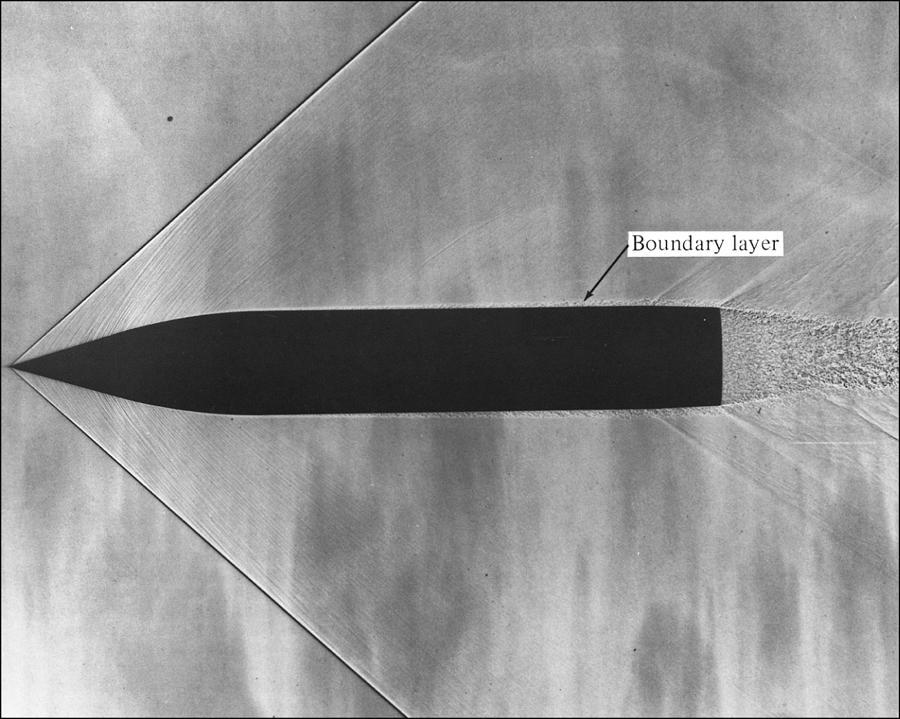
\includegraphics[width=0.9\textwidth]{Motivation/boundary_layer.png}\\
Boundary layer
\end{figure}
\end{column}
\end{columns}
\end{frame}  

% \section{Overview of DPG}
% \subsection{Most Stable Petrov-Galerkin Method}
% \subsection{Minimum Residual Method}
% \section{Motivation}
% \subsection{DPG for CFD}
% \subsubsection{Coarse Mesh Simulation}
% \subsection{DPG for HPC}
% \subsection{Space-Time DPG}
% \subsubsection{Heat Equation}
% \subsubsection{Compressible Navier-Stokes}

% \section{Motivation}
% \subsection{Mesh Generation}
% \subsection{Other Methods}

% \section{Overview of DPG}
% \subsection{Minimum Residual Method}
% \subsection{Mixed Method}
% \subsection{Multiscale Method}
% ------------------------------------------------------------
% \begin{frame}[t]
% \frametitle{Motivation}
% \framesubtitle{DPG Summary}
% Overview of Features
% \begin{itemize}
% \item Robust for singularly perturbed problems
% \item Stable in the preasymptotic regime
% \item Designed for adaptive mesh refinement
% \item Ideal for high-performance computing
% \item DPG is an optimal Petrov-Galerkin method
% \end{itemize}
% \medskip
% DPG is a minimum residual method:
% \[
% u_{h} = \underset{w_{h} \in U_{h}} \argmin \,\, \frac{1}{2}
% \norm{Bw_{h}-l}_{V'}^{2}
% \]
% \vspace{-1em}
% \[
% \scalebox{1.8}{\ensuremath{\Updownarrow}}
% \]
% \vspace{-1em}
% \[
% b(u_h,R_V^{-1}B\delta u_h)
% =l(R_V^{-1}B\delta u_h)
% \quad\forall\delta u_h\in U_h
% \]
% \vspace{-2ex}

% where $v_{\delta u_h}:=R_V^{-1}B\delta u_h$ are the
% \textcolor{utblack}{\textbf{optimal test functions}}.

% % \vspace{4ex}
% % For each $\delta u_h\in U_h$ find $\vdeltau\in V$ such that
% % \[
% % \LRp{\vdeltau,w}_V=b(u,w)\quad\forall w\in V
% % \]
% % where $V$ becomes $V_{p+\Delta p}$ in order to make this computationally tractable.
% \end{frame}


% ------------------------------------------------------------
\begin{frame}[t]
\frametitle{Motivation}
\framesubtitle{Dual Minimum Residual Method}
Find $u\in U$ such that
\[
b(u,v)=l(v)\quad\forall v\in V
\]
with operator $B:U\rightarrow V'$ defined by $b(u,v)=\LRa{Bu,v}_{V'\times V}$.

This give the operator equation 
\[
Bu=l\quad\in V'\,.
\]
We wish to minimize the residual $Bu-l\in V'$:
\[
u_h=\argmin_{w_h\in U_h}\frac{1}{2}\norm{Bu-l}^2_{V'}\,.
\]
Dual norms are not computationally tractable. 
Inverse Riesz map moves the residual to a more accessible space:
\[
u_h=\argmin_{w_h\in U_h}\frac{1}{2}\norm{R_V^{-1}(Bu-l)}^2_{V}\,.
\]
\end{frame}


% ------------------------------------------------------------
\begin{frame}[t]
\frametitle{Motivation}
\framesubtitle{Optimal Petrov-Galerkin Methods}
Taking the G\^ateaux derivative to be zero in all directions $\delta u \in
U_h$ gives,
\[
\left(R_V^{-1}(Bu_h-l),R_V^{-1}B\delta u\right)_V = 0, \quad \forall \delta u \in U,
\]
which by definition of the Riesz map is equivalent to 
\begin{equation*}
\LRa{Bu_h-l,R_V^{-1}B\delta u_h}=0\quad\forall\delta u_h\in U_h\,,
\end{equation*}
with optimal test functions $v_{\delta u_h}\coloneqq R_V^{-1}B\delta u_h$ for each trial function $\delta u_h$.
\begin{block}{Optimal Petrov-Galerkin System}
This gives a simple bilinear form
\begin{equation*}
b(u_h,v_{\delta u_h})=l(v_{\delta u_h}),
\end{equation*}
with $v_{\delta u_h}\in V$ that solves the auxiliary problem
\begin{equation*}
\LRp{v_{\delta u_h},\delta v}_V=\LRa{R_Vv_{\delta u_h},\delta v}
=\LRa{B\delta u_h,\delta v}=b(\delta u_h,\delta v)\quad\forall\delta v\in V.
\end{equation*}
\end{block}
\end{frame}


% ------------------------------------------------------------
\begin{frame}[t]
\frametitle{Motivation}
\framesubtitle{The Most Stable Petrov-Galerkin Method}
Babu\v{s}ka's theorem\cite{Babuska70} guarantees that \emph{discrete stability and approximability imply convergence}.
If bilinear form $b(u,v)$, with $M:=\norm{b}$ satisfies the discrete inf-sup condition 
with constant $\gamma_h$,
\[
\sup_{v_h\in V_h}\frac{|b(u,v)|}{\norm{v_h}_V}\geq\gamma_h\norm{u_h}_U\,,
\]
then the Galerkin error satisfies the bound
\[
\norm{u_h-u}_U\leq\frac{M}{\gamma_h}\inf_{w_h\in U_h}\norm{w_h-u}_U\,.
\]
Optimal test function realize the supremum such that $\gamma_h\geq\gamma$.\\
\begin{block}{Optimal Error Estimates}
If we use the energy norm in the error estimate, then $\norm{b}=\gamma=1$.
Babu\v{s}ka's theorem
implies that the optimal Petrov-Galerkin method is the most stable Petrov-Galerkin method.
\end{block}
\end{frame}


% ------------------------------------------------------------
\begin{frame}[t]
\frametitle{Motivation}
\framesubtitle{The \emph{Discontinuous} Petrov-Galerkin Method}
A continuous test space would produce a globally coupled auxiliary problem.\\
Goal is solve for optimal test functions in an embarrassingly parallel fashion.
\end{frame}


% ------------------------------------------------------------
\begin{frame}[t]
\frametitle{Motivation}
\framesubtitle{Initial mesh design is expensive and time-consuming}
\begin{columns}[t]
\begin{column}[c]{0.4\textwidth}
\begin{itemize}
  \item Surface mesh must accurately represent geometry
  \item Volume mesh needs sufficient resolution for asymptotic regime
  % Before we accurately know the flow features
  \item Boundary layer meshes must respect $y^+$ guidelines
  \item Engineers often forced to work by trial and error
  \item Bad in the context of HPC
\end{itemize}
\end{column}
\begin{column}[c]{0.6\textwidth}
\vspace{2ex}
\begin{figure}[t]
\centering
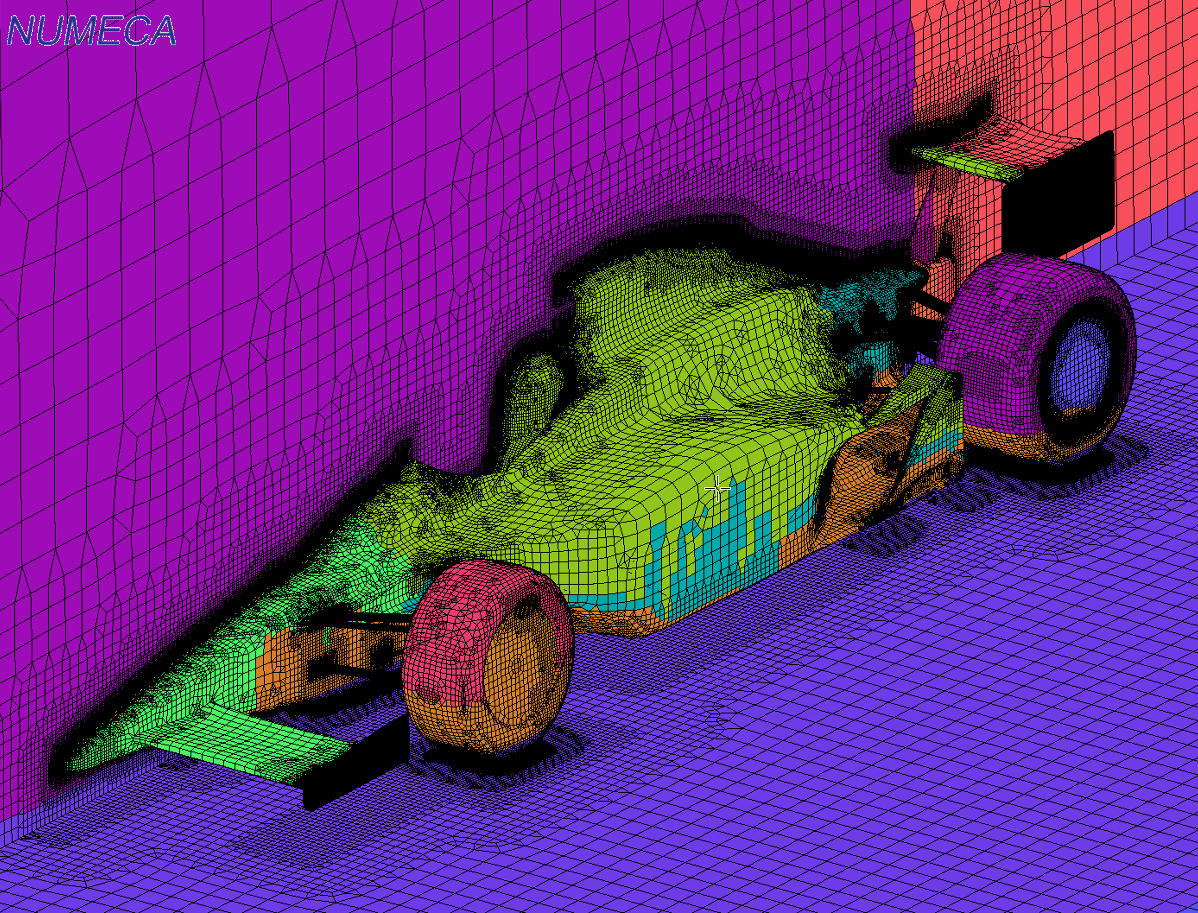
\includegraphics[width=1.0\textwidth]{Motivation/NumecaRaceCar.png}
\\\small{Formula 1 Mesh by Numeca}\\
\end{figure}
\end{column}
\end{columns}
\end{frame}

% ------------------------------------------------------------
\begin{frame}[t]
\frametitle{Adaptive Mesh Refinement from Coarse Meshes}
\framesubtitle{Adaptive solve of the Carter plate problem}
\foreach \n in {1,...,11}
{
\only<\n>
{
\begin{figure}[ht]
\centering
\begin{subfigure}[c]{0.45\textwidth}
\centering
\includegraphics[width=0.99\textwidth]{Motivation/Plate/u\n.png}\\
\vspace{-1ex}
{\scriptsize Velocity}\\
\end{subfigure}
\begin{subfigure}[c]{0.45\textwidth}
\centering
\includegraphics[width=0.99\textwidth]{Motivation/Plate/T\n.png}\\
\vspace{-1ex}
{\scriptsize Temperature}\\
\end{subfigure}
\begin{subfigure}[c]{0.5\textwidth}
\centering
\vspace{2ex}
\includegraphics[width=0.99\textwidth]{Motivation/Plate/mesh\n.png}\\
\vspace{-1ex}
{\scriptsize Mesh \n}\\
\end{subfigure}
\end{figure}
}
}
\end{frame}



% ------------------------------------------------------------
% \begin{frame}[t]
% \frametitle{Motivation}
% \framesubtitle{DPG for Massively Parallel CFD}  %% needed for proper positioning of the logo ...
% Pre-asymptotic stability and automatic adaptivity make a powerful synthesis.
% \begin{itemize}
%   \item Initial mesh design is a time consuming and expensive part of CFD.
%   \item Pre-asymptotic stability allows a DPG simulation to begin on the coarsest possible mesh.
%   \item Many methods become unstable in the pre-asymptotic regime.
%   \item Human intervention to correct a failed massively parallel simulation can be very costly.
%   \item Error indicator function indicates targets most important areas for refinement.
%   \item Provably robust for singularly perturbed problems.
% \end{itemize}

% \vspace{2ex}
% Space-time DPG extends these benefits to transient problems.
% \begin{itemize}
%   \item Localizes temporal adaptivity similar to spatial adaptivity.
% \end{itemize}
% \end{frame}




%   /$$        /$$$$$$ 
%  | $$       /$$__  $$
%  | $$      | $$  \__/
%  | $$      | $$      
%  | $$      | $$      
%  | $$      | $$    $$
%  | $$$$$$$$|  $$$$$$/
%  |________/ \______/ 
%                      
%                      
%      
\section{Locally Conservative DPG}
% \subsection{Mathematics}
% \subsection{Numerical Results}
%===============================================================================
% NEW SLIDE
%===============================================================================
\begin{frame}
\frametitle{Locally Conservative DPG}
\framesubtitle{DPG for Convection-Diffusion}
Start with the strong-form PDE.
\[
\nabla\cdot(\bfbeta u)-\epsilon\Delta u = g
\]
Rewrite as a system of first-order equations.
\begin{align*}
\nabla\cdot(\bfbeta u-\bfsigma)&=g\\
\frac{1}{\epsilon}\bfsigma-\nabla u&=\boldsymbol0
\end{align*}
Multiply by test functions and integrate by parts over each element, $K$.
\begin{align*}
-(\bfbeta u-\bfsigma,\nabla v)_K+((\bfbeta
u-\bfsigma)\cdot\mathbf{n},v)_{\partial K}&=(g,v)_K\\
\frac{1}{\epsilon}(\bfsigma,\bftau)_K+(u,\nabla\cdot\bftau)_K
-(u,\tau_n)_{\partial K}&=0
\end{align*}
Use the ultraweak (DPG) formulation to obtain bilinear form $b(u,v)=l(v)$.
\begin{align*}
-(\bfbeta u-\bfsigma,\nabla v)_K&+(\hat f,v)_{\partial K}
+ \frac{1}{\epsilon}(\bfsigma,\bftau)_K\\
&+(u,\nabla\cdot\bftau)_K
-(\hat u,\tau_n)_{\partial K}=(g,v)_K
\end{align*}
\end{frame}
\begin{comment}
With that ultra-brief refresher, we can now apply DPG to the
convection-diffusion equation. We prefer to work with systems of first order
equations. Then, multiplying the top equation by a scalar valued test
function, v, and the second by a vector valued test function tau, we can
integrate by parts over each element, K. Combining the two equations, we get
our bilinear form for convection diffusion. We seek the field variable, u and
sigma in L2, but that leaves their traces undefined. So, in a manner similar
to the hybridized DG method, we define new unknowns for our traces and fluxes,
u hat and f hat.
\end{comment}


%    /$$$$$$                                                                           /$$     /$$                     
%   /$$__  $$                                                                         | $$    |__/                     
%  | $$  \__/  /$$$$$$  /$$$$$$$   /$$$$$$$  /$$$$$$   /$$$$$$  /$$    /$$  /$$$$$$  /$$$$$$   /$$ /$$    /$$  /$$$$$$ 
%  | $$       /$$__  $$| $$__  $$ /$$_____/ /$$__  $$ /$$__  $$|  $$  /$$/ |____  $$|_  $$_/  | $$|  $$  /$$/ /$$__  $$
%  | $$      | $$  \ $$| $$  \ $$|  $$$$$$ | $$$$$$$$| $$  \__/ \  $$/$$/   /$$$$$$$  | $$    | $$ \  $$/$$/ | $$$$$$$$
%  | $$    $$| $$  | $$| $$  | $$ \____  $$| $$_____/| $$        \  $$$/   /$$__  $$  | $$ /$$| $$  \  $$$/  | $$_____/
%  |  $$$$$$/|  $$$$$$/| $$  | $$ /$$$$$$$/|  $$$$$$$| $$         \  $/   |  $$$$$$$  |  $$$$/| $$   \  $/   |  $$$$$$$
%   \______/  \______/ |__/  |__/|_______/  \_______/|__/          \_/     \_______/   \___/  |__/    \_/     \_______/
%                                                                                                                      
%                                                                                                                      
%     
%===============================================================================
% NEW SLIDE
%===============================================================================
\begin{frame}
\frametitle{Locally Conservative DPG}
\framesubtitle{Local conservation for convection-diffusion}
The local conservation law in convection diffusion is
\[
\int_{\partial K}\hat f=\int_K g\,,
\]
which is equivalent to having $\mathbf{v}_K:=\{v,\bftau\}=\{1_K,\boldsymbol0\}$ in the test space.
In general, this is not satisfied by the optimal test functions.
Following Moro et al\textsuperscript{\cite{MoroNguyenPeraire11}} (also
Chang and Nelson\textsuperscript{\cite{ChangNelson1997}}), we
can enforce this condition with Lagrange multipliers:
\begin{align*}
L(u_h,\bflambda) = \frac{1}{2}\norm{R_V^{-1}(Bu_h-l)}_V^2
-\sum_K\lambda_K\underbrace{\langle Bu_h-l,\mathbf{v}_K\rangle}_
{\langle\hat f, 1_K\rangle_{\partial K}-\langle g,1_K\rangle_K}\,,
\end{align*}
where $\bflambda=\{\lambda_1,\cdots,\lambda_N\}$.
\end{frame}
\begin{comment}
So what does local conservation mean for the convection-diffusion equation. We
want the integral of our fluxes over the element faces to be balanced by any
source terms in the RHS. This is equivalent to having one in the test space.
You can see this if you look at the bilinear form on the previous slide and
plug one and zero in as test functions. Unfortunately the optimal test
functions do not always span constants. It turns out we can augment our test
space with constants through the use of Lagrange multipliers. So taking a
couple of steps backward in the abstract form, we can augment our system with
the Lagrange multipliers enforcing local conservation.
\end{comment}


%===============================================================================
% NEW SLIDE
%===============================================================================
\begin{frame}
\frametitle{Locally Conservative DPG}
\framesubtitle{Locally Conservative Saddle Point System}
Finding the critical points of $L(u,\bflambda)$, we get the following
equations\textsuperscript{\cite{EllisDemkowiczChan2013}}.
\begin{align*}
\frac{\partial L(u_h,\bflambda)}{\partial u_h}&=b(u_h,R_V^{-1}B\delta u_h)
-l(R_V^{-1}B\delta u_h)\\
&{\color{red}-\sum_K\lambda_K b(\delta
u_h,\mathbf{v}_K)}=0\quad\forall\delta u_h\in U_h
\end{align*}
\[
\frac{\partial
L(u_h,\bflambda)}{\partial\lambda_K}=-b(u_h,\mathbf{v}_K)+l(\mathbf{v}_K)=0\quad\forall
K
\]
A few consequences:
\begin{itemize}
\item We've turned our minimization problem into a saddlepoint problem.
% \item New $\lambda_K$ DOFs can be statically condensed out.
\item Only need to find the optimal test function in the orthogonal complement
of constants. % Backup slide
\end{itemize}
\end{frame}
\begin{comment}
Now, proceeding forward again and setting the derivatives to zero, we have
turned our minimization problem into a saddle point problem. Note that we have
added extra DOFs equal to the number of mesh elements, but the structure of
the problem allows these to be statically condensed out. The most interesting
consequence of this modification (apart from enforcing local conservation) is
that we can modify the search space for our optimal test functions to be
the orthogonal complement of constants.
\end{comment}


%===============================================================================
% NEW SLIDE
%===============================================================================
\begin{frame}
\frametitle{Locally Conservative DPG}
\framesubtitle{Optimal Test Functions}
For each $\mathbf{u}=\{u,\bfsigma,\hat u,\hat f\}\in\mathbf{U}_h$, find
$\mathbf{v}_{\mathbf{u}}=\{v_\mathbf{u},\bftau_\mathbf{u}\}\in\mathbf{V}$ such that
\[
(\mathbf{v_u},\mathbf{w})_\mathbf{V}=b(\mathbf{u},\mathbf{w})\quad\forall\mathbf{w}\in\mathbf{V}
\]
where $\mathbf{V}$ becomes $\mathbf{V}_{p+\Delta p}$ in order to make this
computationally tractable.

We recently developed this modification to the \emph{robust test norm}
\textsuperscript{\cite{ChanHeuerThanhDemkowicz2012}} which behaves better in
the presence of singularities.
\begin{minipage}[t][1.5in]{\textwidth}
\begin{align*}
\norm{(v,\bftau)}^2_{\mathbf{V},\Omega_h}&=
\norm{\min\left\{\frac{1}{\sqrt{\epsilon}},\frac{1}{\sqrt{|K|}}\right\}\bftau}^2
+\norm{\nabla\cdot\bftau-\bfbeta\cdot\nabla v}^2\\
&+\norm{\bfbeta\cdot\nabla v}^2+\epsilon\norm{\nabla v}^2
\underbrace{\color{red}{
\begin{minipage}[c][0.3in][c]{0.9in}$
\only<1>{
\hspace{1.5ex}
+\norm{v}^2
}
\only<2>{
+\left(\frac{1}{|K|}\int_Kv\right)^2
}$
\end{minipage}
}}_{\only<1>{\text{No longer necessary}}\only<2>{\text{Zero mean term}}}
\end{align*}
\end{minipage}
\end{frame}
\begin{comment}
So how does this affect our search for optimal test functions? The process to
compute optimal test functions is as follows. For each trial function we are
considering, we want to find the test function in an enriched space that
satisfies the following relation - that the inner product of vu with w equals
the bilinear form acting on u and w for all w in V.

The choice of norm on V can significantly affect the robustness of the
solution. Unfortunately, the optimal test norm is not localizable, and for
convection diffusion, the quasi-optimal test norm has boundary layers arising
from the adjoint and thus has approximability issues. Fortunately a
couple of collaborators developed a robust test norm for convection-diffusion.
Sadly, this norm also has its issues as the final zero order term in the
expression is somewhat troublesome. (???)

Why can we replace the L2 term with the zero mean term?
Why is zero mean more friendly than L2?
- Not mesh dependent
- No boundary layers
\end{comment}


%    /$$$$$$    /$$               /$$       /$$ /$$ /$$   /$$              
%   /$$__  $$  | $$              | $$      |__/| $$|__/  | $$              
%  | $$  \__/ /$$$$$$    /$$$$$$ | $$$$$$$  /$$| $$ /$$ /$$$$$$   /$$   /$$
%  |  $$$$$$ |_  $$_/   |____  $$| $$__  $$| $$| $$| $$|_  $$_/  | $$  | $$
%   \____  $$  | $$      /$$$$$$$| $$  \ $$| $$| $$| $$  | $$    | $$  | $$
%   /$$  \ $$  | $$ /$$ /$$__  $$| $$  | $$| $$| $$| $$  | $$ /$$| $$  | $$
%  |  $$$$$$/  |  $$$$/|  $$$$$$$| $$$$$$$/| $$| $$| $$  |  $$$$/|  $$$$$$$
%   \______/    \___/   \_______/|_______/ |__/|__/|__/   \___/   \____  $$
%                                                                 /$$  | $$
%                                                                |  $$$$$$/
%                                                                 \______/ 
%===============================================================================
% NEW SLIDE
%===============================================================================
\begin{frame}
\frametitle{Locally Conservative DPG}
\framesubtitle{Stability Analysis}
We follow Brezzi's theory for an abstract mixed problem:
\begin{equation*}
\left\{
\begin{array}{lll}
\bfu \in \bfU, p \in Q\\
a(\bfu,\bfw) + c(p,\bfw) & = l(\bfw) & \forall \bfw \in \bfU \\
c(q,\bfu) & = g(q) & \forall q \in Q
\end{array}
\right.
\end{equation*}
where $a,c,l,g$ denote the appropriate
bilinear and linear forms. Note that
$a(\bfu,\bfw)=b(\bfu,R_V^{-1}B\bfw)=(R_V^{-1}B\bfu,R_V^{-1}B\bfw)_V$.

Let $\bfpsi$ denote the $\bfH(\text{div},\Omega)$ extension of flux $\hat{f}$
that realizes the minimum in the definition of the quotient (minimum energy
extension) norm.

The norm for the Lagrange multipliers $\lambda_K$ is implied
by the quotient norm used for $H^{-1/2}(\Gamma_h)$ and continuity
bound for form $c(p,\bfw)$:
\[
||\bflambda||:=\left(\sum_K \mu(K) \lambda_K^2\right)^{1/2}
\]
\end{frame}
\begin{comment}
In the following analysis, we neglect the error due to the approximation of optimal test functions.

We skip some of the math needed to show this, but it is pretty trivial. The
full details will be in the ICES report.
\end{comment}


%===============================================================================
% NEW SLIDE
%===============================================================================
\begin{frame}
\frametitle{Locally Conservative DPG}
\framesubtitle{Inf Sup Condition}
\only<1>{
The inf-sup condition relating spaces $\bfU$ and $Q$ is
\[
\sup_{\bfw \in \bfU} \frac{| c(p,\bfw) |}{|| \bfw ||_{\bfU}} \geq \beta ||
p ||_Q
\]
Let
\begin{equation*}
R\, : \, L^2(\Omega) \ni q \to \bfpsi \in \bfH(\text{div},\Omega) \cap \bfH^1(\Omega)
=\bfH^1(\Omega)
\end{equation*}
be
the continuous right inverse of the divergence operator constructed by
Costabel and McIntosh\textsuperscript{\cite{CostabelMcIntosh}}.
Let $\bfpsi_h$ denote the classical, lowest order Raviart-Thomas (RT) interpolant of
function
\begin{equation*}
\bfpsi = R (\sum_K \lambda_K 1_K)
\end{equation*}
Note that $\text{div} \bfpsi_h = \text{div} \bfpsi = \lambda_K$ in element $K$.
}
\only<2>{
Classical $h$-interpolation error estimate for the lowest error
Raviart-Thomas elements and continuity of operator $R$ imply the stability estimate:
\begin{equation*}
\begin{array}{lll}
|| \bfpsi_h || & \leq || \bfpsi_h - \bfpsi || + || \bfpsi ||\\[8pt]
&\leq C h || \bfpsi ||_{H^1} +  || \bfpsi || \\[8pt]
& \leq C || \text{div} \bfpsi || = C (\sum_K \mu(K) \lambda_K^2)^{1/2}
\end{array}
\end{equation*}
Let $\hat{f}$ be the trace of $\bfpsi_h$, then
\begin{align*}
\sup_{\hat{f} \in H^{-1/2}(\Gamma_h)} \frac{|  \sum_K \lambda_K \langle
\hat{f},1_K \rangle_{\partial K} |}{|| \hat{f} ||_{H^{-1/2}(\Gamma_h)}}
&\geq \frac{| \sum_K \lambda_K \int_K \text{div} \bfpsi_h \: 1_K  |}
{|| \bfpsi_h ||_{H(\text{div},\Omega)}}\\
&\geq \frac{1}{C} (\sum_K \mu(K) \lambda_K^2)^{1/2}
\end{align*}
}
\end{frame}
\begin{comment}
We proceed now with the discussion of the discrete inf-sup stability
constants. We skip index h in the notation.

Note that C is a generic, mesh independent constant incorporating the constant
from the interpolation error estimate and the continuity constant of R.

Notice that we have considered traces of lowest order Raviart-Thomas elements
for the discretization of the flux.

The inf-sup condition for the lowest order RT spaces implies automatically the
analogous condition for elements of arbitrary order; increasing space U only
makes the discrete inf-sup constant bigger.
\end{comment}


%===============================================================================
% NEW SLIDE
%===============================================================================
\begin{frame}
\frametitle{Locally Conservative DPG}
\framesubtitle{Inf Sup in Kernel Condition}
We characterize the ``kernel'' space:
\begin{equation*}
\begin{array}
{rl}
\bfU_0  := & \{ \bfw \in \bfU \, : \, c(q,\bfw) = 0 \quad \forall q \in Q\} \\[8pt]
 = &\{ (u,\bfsigma,\hat{u},\hat{t}) \, : \, \langle \hat{t},1_K \rangle = 0
 \quad \forall K \}
\end{array}
\end{equation*}
With $\bfu \in \bfU_0$, we have then:
\begin{align*}
   \sup_{\bfw \in \bfU_0} \frac{| a(\bfu,\bfw) |}{|| \bfw ||_{\bfU} }
   &\geq \frac{| b(\bfu,T \bfu) |}{|| \bfu ||}
   = \frac{| b(\bfu,T \bfu) |}{|| T\bfu ||}\frac{||T\bfu||}{||\bfu||}\\
   &= \sup_{(v,\bftau)}\frac{| b((u,\bfsigma,\hat{u},\hat{t}), (v,\bftau)) |}{|| (v,\bftau) ||}
   \frac{||T\bfu||}{||\bfu||}
   \geq \gamma^2 || (u,\bfsigma,\hat{u},\hat{t}) ||
\end{align*}
where $\gamma$ is the stability constant for the standard DPG formulation.

The FE error is bounded by the best approximation error. Note that the exact
Lagrange multipliers are zero, so the best approximation error involves only
the solution $(u,\bfsigma,\hat{u},\hat{t})$.
\end{frame}
\begin{comment}
This is satisfied automatically due to the use of optimal test functions.

In other words, the kernel space contains only the equilibrated fluxes.

The first inequality follows as we plug in the definition for a and pick w=u.
The second equality is trivial, while the next one follows by definition of
the optimal test functions given through the trial-to-test operator T .
\end{comment}


%   /$$$$$$$            /$$                             /$$                                            
%  | $$__  $$          | $$                            | $$                                            
%  | $$  \ $$  /$$$$$$ | $$$$$$$  /$$   /$$  /$$$$$$$ /$$$$$$   /$$$$$$$   /$$$$$$   /$$$$$$$  /$$$$$$$
%  | $$$$$$$/ /$$__  $$| $$__  $$| $$  | $$ /$$_____/|_  $$_/  | $$__  $$ /$$__  $$ /$$_____/ /$$_____/
%  | $$__  $$| $$  \ $$| $$  \ $$| $$  | $$|  $$$$$$   | $$    | $$  \ $$| $$$$$$$$|  $$$$$$ |  $$$$$$ 
%  | $$  \ $$| $$  | $$| $$  | $$| $$  | $$ \____  $$  | $$ /$$| $$  | $$| $$_____/ \____  $$ \____  $$
%  | $$  | $$|  $$$$$$/| $$$$$$$/|  $$$$$$/ /$$$$$$$/  |  $$$$/| $$  | $$|  $$$$$$$ /$$$$$$$/ /$$$$$$$/
%  |__/  |__/ \______/ |_______/  \______/ |_______/    \___/  |__/  |__/ \_______/|_______/ |_______/ 
%                                                                                                      
%                                                                                                      
%  
%===============================================================================
% NEW SLIDE
%===============================================================================
\begin{frame}
\frametitle{Locally Conservative DPG}
\framesubtitle{Robustness Analysis}
\begin{itemize}
  \item We prove robustness of the restricted DPG method by switching to the
    energy norm in Brezzi's stability analysis.
  \item The inf-sup in kernel condition is simple. Upon replacing the original
    norm of solution $\bfu$ with the energy norm, $\gamma$ and the continuity
    constant become one.
  \item In order to investigate the robustness of inf-sup constant $\beta$, we
    need to understand what the energy norm of flux variable $\hat f$ is.
  \item For an element, $K$, we solve for the optimal test functions,
    $v_K\in H^1(K)$, and $\bftau_K\in\bfH(\text{div},K)$
    corresponding to flux $\hat f$:
    \[
    ( (v_K,\bftau_K),(\delta v,\delta\bftau) )_V=\LRa{\hat f,\delta v}
    \quad\forall\delta v\in H^1(K),\,\delta\bftau\in\bfH(\text{div},K)
    \]
  \item The energy norm for $\hat f$ is then
    \[
    ||\hat f||_E^2=\sum_K||(v_K,\bftau_K)||_V^2
    \]
\end{itemize}
\end{frame}
\begin{comment}
  With robust test norms, standard DPG delivers a robust error bound because
  it minimizes the residual in the energy norm. Restricted DPG no longer
  minimizes the residual, so can we claim robustness for this version as well?
\end{comment}


%===============================================================================
% NEW SLIDE
%===============================================================================
\begin{frame}
\frametitle{Locally Conservative DPG}
\framesubtitle{Robustness Analysis}
\begin{itemize}
    \item Need to establish conditions under which the inf-sup constant is
      independent of viscosity.
      \begin{equation*}
        \sup_{\hat{f}} \frac{| \sum_K \lambda_K \langle \hat{f},1_K \rangle |}{|| \hat{f} ||_E}
        \geq  \beta \LRp{\sum_K \mu(K) \lambda_K^2}^{1/2}
      \end{equation*}
    \item Select $\hat f$ as the trace of the Raviart-Thomas interpolant
      $\bfpsi_h$ of $\bfpsi=R(\sum_K\lambda_K1_K)$.
    \item Proceed as in the previous analysis, but evaluation of the norm of
      $\hat f$ requires a local solve.
      \begin{align*}
        ( (v,\bftau),&(\delta v,\delta\bftau) )_V
        =\LRa{\hat f,\delta v}_{\partial K}
        =\int_K\text{div}\bfpsi_h\delta v
        =\int_K\text{div}\bfpsi\delta v\\
        &=\int_K\lambda_K\delta v=\lambda_K(1_K,\delta v)_K
        \quad\forall\delta v\in
        H^1(K)\,\forall\delta\bftau\in\bfH(\text{div},K)
      \end{align*}
\end{itemize}
\end{frame}
\begin{comment}
We need to establish sufficient conditions under which the inf-sup and continuity constants for the bilinear
form representing the constraint are independent of viscosity

R is the right inverse of the divergence operator constructed by Costabel and
McIntosh.
\end{comment}


%===============================================================================
% NEW SLIDE
%===============================================================================
\begin{frame}
\frametitle{Locally Conservative DPG}
\framesubtitle{Robustness Analysis}
\begin{itemize}
    \item We need an upper bound for the energy norm of $(v_h,\bftau_h)$:
      \[
      \LRp{\sum_K||(v,\bftau)||^2_V}^{1/2}
      \]
    \item Substituting $(v,\bftau)$ for $(\delta v,\delta\bftau)$ in the
      previous slide:
      \[
      ||(v,\bftau)||^2_V=\lambda_K(1_K,v_k)
      \]
    \item With a robust stability estimate
      $
      (1_K,v_K)\leq C\mu(K)^{1/2}||(v,\bftau)||_K\,,
      $
      \[
      ||(v,\bftau)||_V\leq C\mu(K)^{1/2}|\lambda_K|
      \]
      \[
      \sum_K||(v,\bftau)||_V^2\leq C^2\sum_K\mu(K)\lambda_K^2
      \]
      which leads to the robust estimate of inf-sup constant $\beta$.
\end{itemize}
\end{frame}
\begin{comment}
\end{comment}


%===============================================================================
% NEW SLIDE
%===============================================================================
\begin{frame}
\frametitle{Locally Conservative DPG}
\framesubtitle{Robustness Analysis}
\begin{itemize}
    \item Finally, we need a continuity estimate on
      \[
      \sum_K\lambda_K\langle\hat f,1_K\rangle
      \]
    \item Testing with $(1_K,\boldsymbol0)$ in the local problem, we obtain
      \[
      ( (v,\bftau),(1_K,\boldsymbol0) )_V=\langle\hat f,1_K\rangle_{\partial K}
      \]
    \item With a robust estimate $|( (v,\bftau),(1_K,\boldsymbol0) )_V|\leq
      C\mu(K)^{1/2}||(v,\bftau)||_V$,
      \begin{align*}
        |\sum_K\lambda_K\langle\hat f,1_K\rangle|
        &\leq C\LRp{\sum_K\mu(K)\lambda_K^2}^{1/2}\LRp{\sum_K||(v,\bftau)||_V^2}^{1/2}\\
        &=C\LRp{\sum_K\mu(K)\lambda_K^2}^{1/2}||\hat f||_E
      \end{align*}
\end{itemize}
\end{frame}
\begin{comment}
With the robust stability and continuity constants for the mixed problem, the
energy error of solution and Lagrange multipliers is bounded robustly by the
best approximation error measured in the energy norm. We arrive thus at the
same situation as in standard DPG.
\end{comment}


%   /$$$$$$$$           /$$           /$$                                    
%  | $$_____/          |__/          | $$                                    
%  | $$        /$$$$$$  /$$  /$$$$$$$| $$   /$$  /$$$$$$$  /$$$$$$  /$$$$$$$ 
%  | $$$$$    /$$__  $$| $$ /$$_____/| $$  /$$/ /$$_____/ /$$__  $$| $$__  $$
%  | $$__/   | $$  \__/| $$| $$      | $$$$$$/ |  $$$$$$ | $$  \ $$| $$  \ $$
%  | $$      | $$      | $$| $$      | $$_  $$  \____  $$| $$  | $$| $$  | $$
%  | $$$$$$$$| $$      | $$|  $$$$$$$| $$ \  $$ /$$$$$$$/|  $$$$$$/| $$  | $$
%  |________/|__/      |__/ \_______/|__/  \__/|_______/  \______/ |__/  |__/
%                                                                            
%                                                                            
%   
%===============================================================================
% NEW SLIDE
%===============================================================================
\begin{frame}
\frametitle{Numerical Experiments}
\framesubtitle{Erickson-Johnson Problem}
On domain $\Omega=[0,1]^2$, with $\beta=(1,0)^T$, $f=0$ and boundary
conditions
\[
\hat f=u_0,\quad\beta_n\le0\,,\quad\quad\hat u=0,\quad\beta_n > 0
\]
Separation of variabes gives an analytic solution
\[
u(x,y)=C_0+\sum_{n=1}^\infty C_n
\frac{\exp(r_2(x-1))-\exp(r_1(x-1))}{r_1\exp(-r_2)-r_2\exp(-r_1)}
\cos(n\pi y)
\]
\vspace{-5ex}
\begin{columns}[b]
\begin{column}{0.5\textwidth}
\begin{figure}[t]
\centering
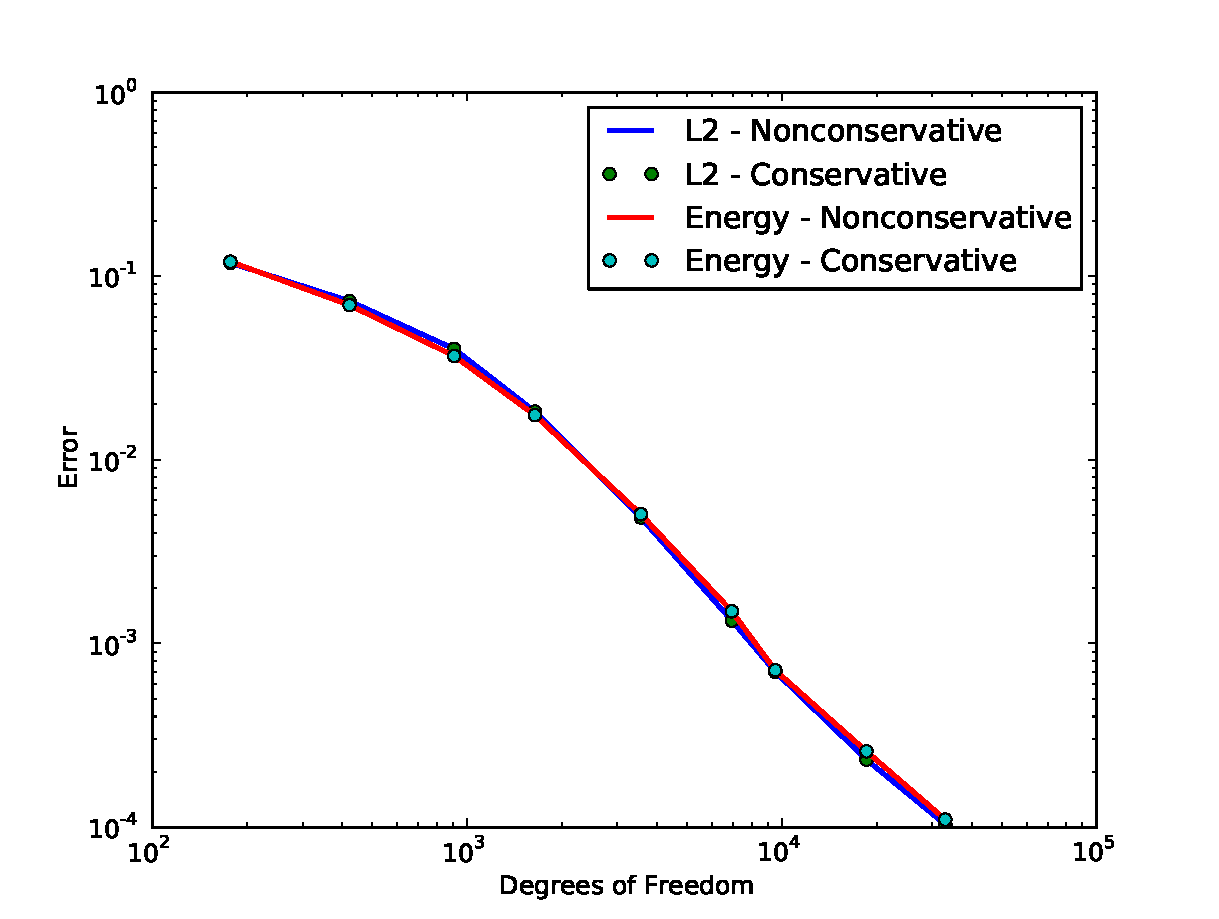
\includegraphics[width=0.9\textwidth]{Erickson/modifiedError.pdf}

\end{figure}
\end{column}
\begin{column}{0.5\textwidth}
\begin{figure}[t]
\centering
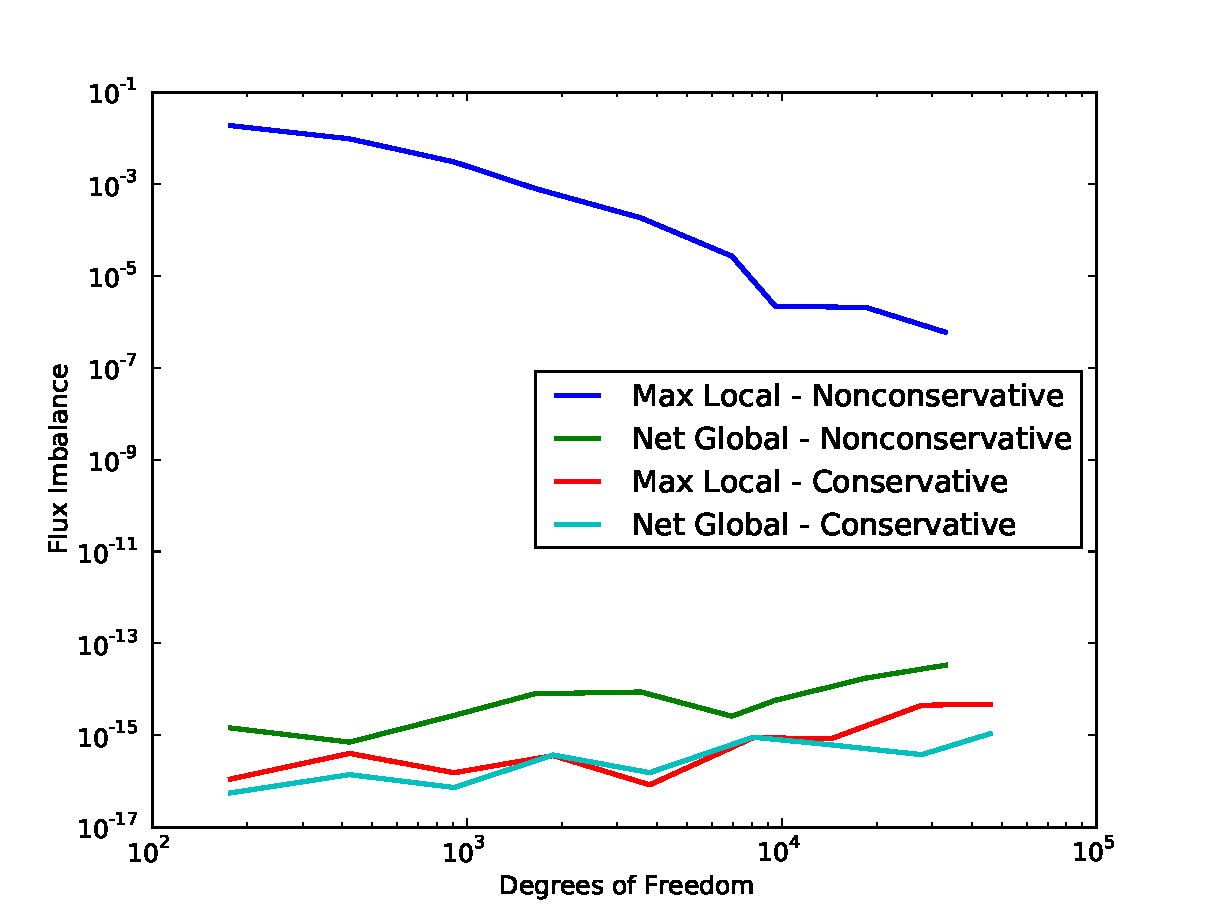
\includegraphics[width=0.9\textwidth]{Erickson/modifiedFlux.pdf}

\end{figure}
\end{column}
\end{columns}
\end{frame}
\begin{comment}
\end{comment}


%    /$$$$$$    /$$               /$$                          
%   /$$__  $$  | $$              | $$                          
%  | $$  \__/ /$$$$$$    /$$$$$$ | $$   /$$  /$$$$$$   /$$$$$$$
%  |  $$$$$$ |_  $$_/   /$$__  $$| $$  /$$/ /$$__  $$ /$$_____/
%   \____  $$  | $$    | $$  \ $$| $$$$$$/ | $$$$$$$$|  $$$$$$ 
%   /$$  \ $$  | $$ /$$| $$  | $$| $$_  $$ | $$_____/ \____  $$
%  |  $$$$$$/  |  $$$$/|  $$$$$$/| $$ \  $$|  $$$$$$$ /$$$$$$$/
%   \______/    \___/   \______/ |__/  \__/ \_______/|_______/ 
%                                                              
%                                                              
%   
%===============================================================================
% NEW SLIDE
%===============================================================================
\begin{frame}
\frametitle{Numerical Experiments}
\framesubtitle{Stokes Flow Around a Cylinder}
\begin{columns}
\begin{column}{0.49\textwidth}
\only<1>{
\begin{figure}
\centering
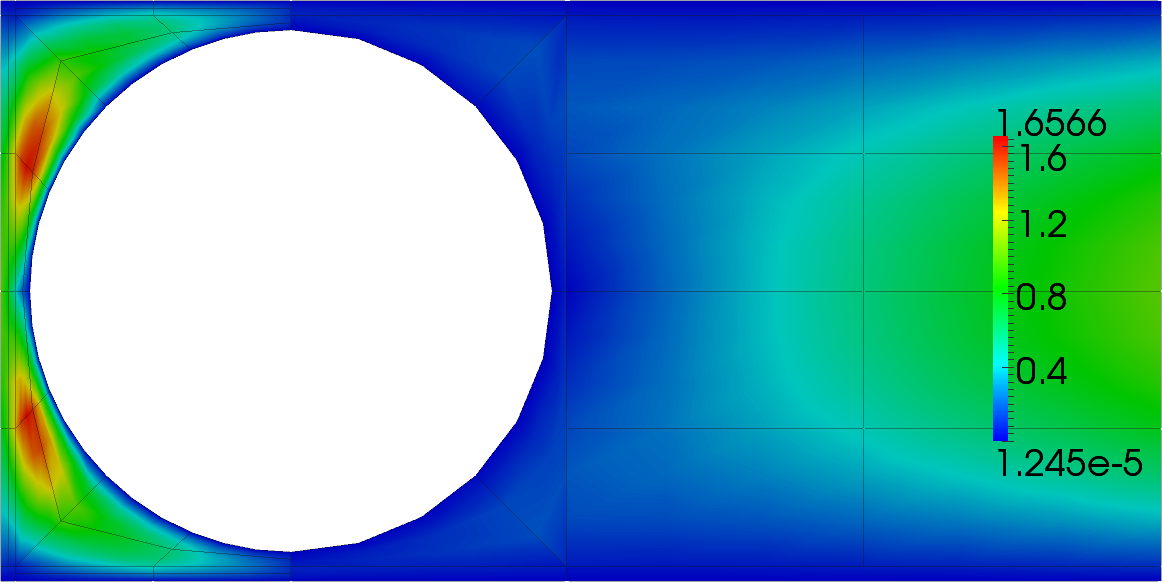
\includegraphics[width=1.0\textwidth]{StokesCylinder/umag9_NC1.png}\\
\vspace{-1ex}
{\scriptsize 1 Refinement}\\
\vspace{1ex}
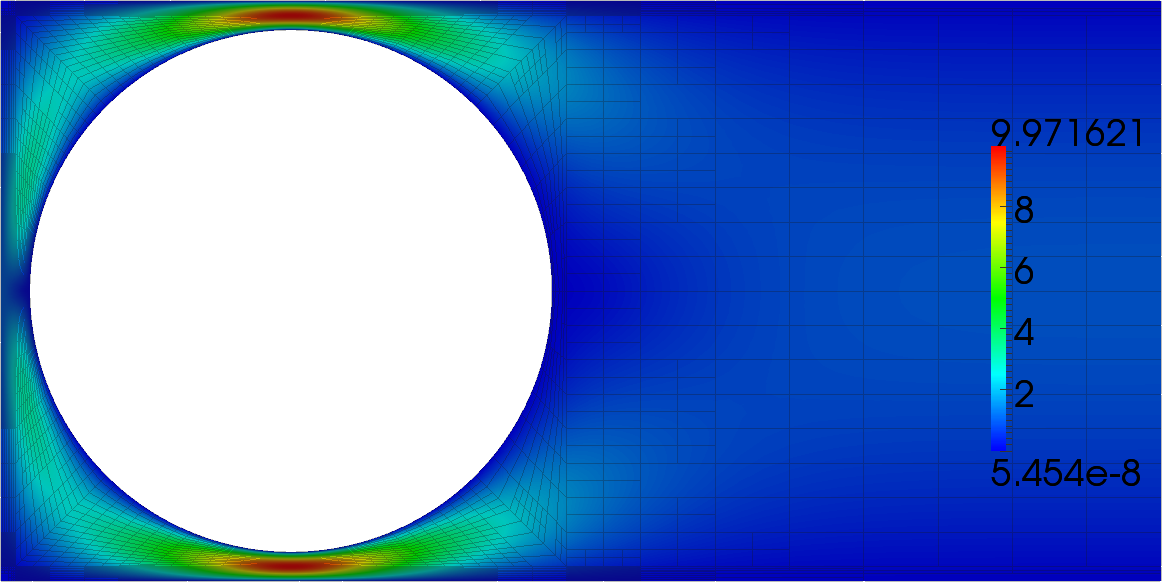
\includegraphics[width=1.0\textwidth]{StokesCylinder/umag9_NC6.png}
\vspace{-1ex}
{\scriptsize 6 Refinements}
\vspace{1ex}

Nonconservative
\end{figure}
\end{column}
\begin{column}{0.49\textwidth}
\begin{figure}
\centering
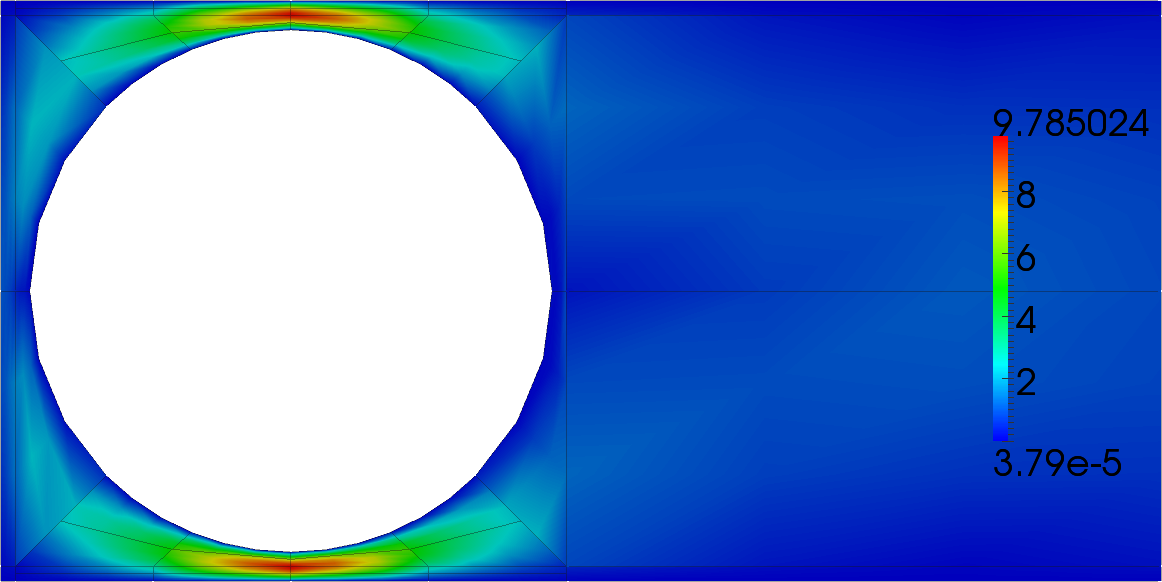
\includegraphics[width=1.0\textwidth]{StokesCylinder/umag9_C1.png}\\
\vspace{-1ex}
{\scriptsize 1 Refinement}\\
\vspace{1ex}
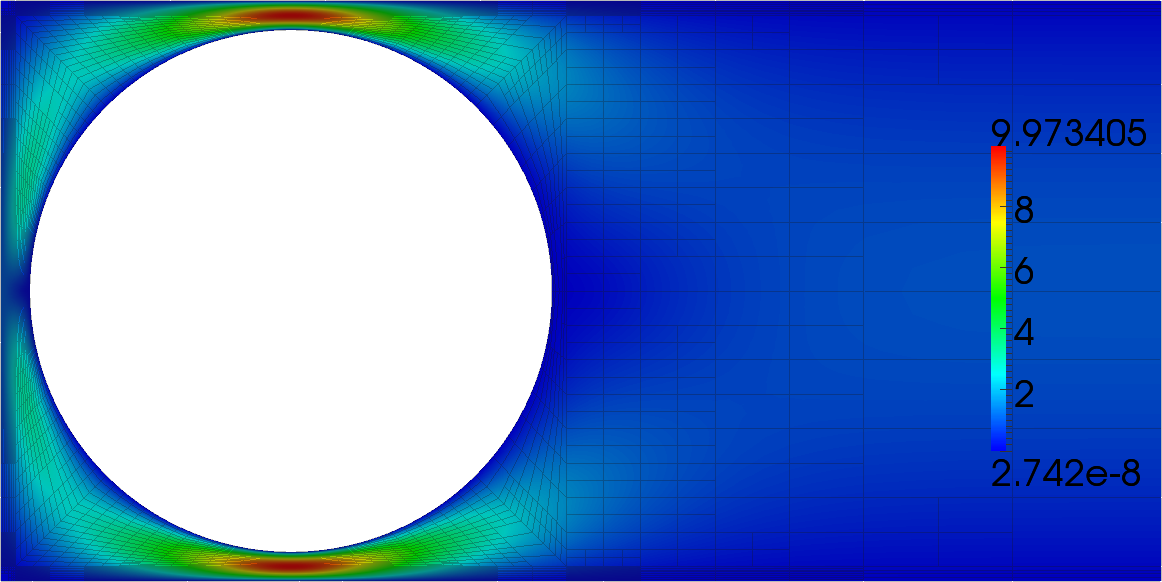
\includegraphics[width=1.0\textwidth]{StokesCylinder/umag9_C6.png}
\vspace{-1ex}
{\scriptsize 6 Refinements}
\vspace{1ex}

Conservative
\end{figure}
}
\only<2>{
\begin{figure}[t]
\centering
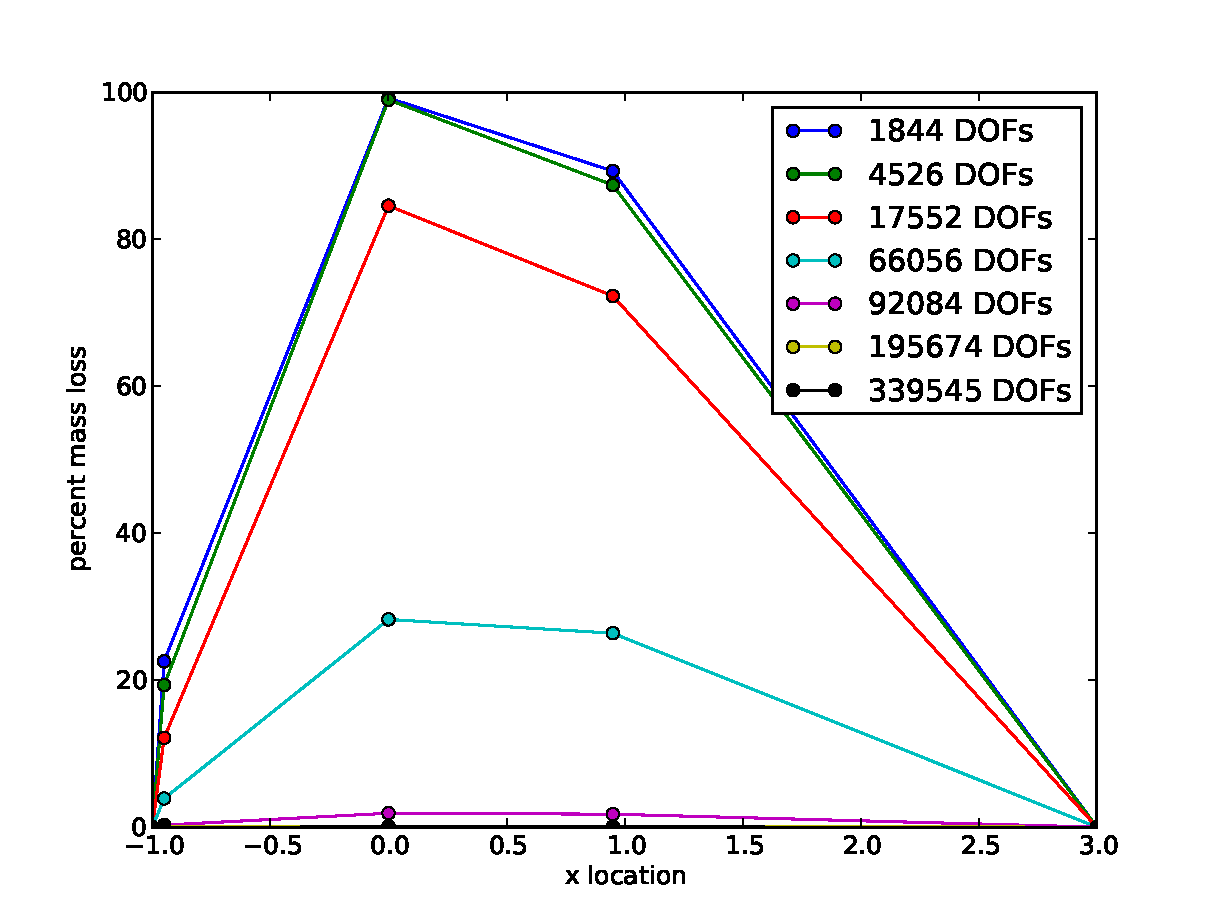
\includegraphics[width=1.1\textwidth]{StokesCylinder/MassLoss9_NC.pdf}

Nonconservative
\end{figure}
\end{column}
\begin{column}{0.49\textwidth}
\begin{figure}[t]
\centering
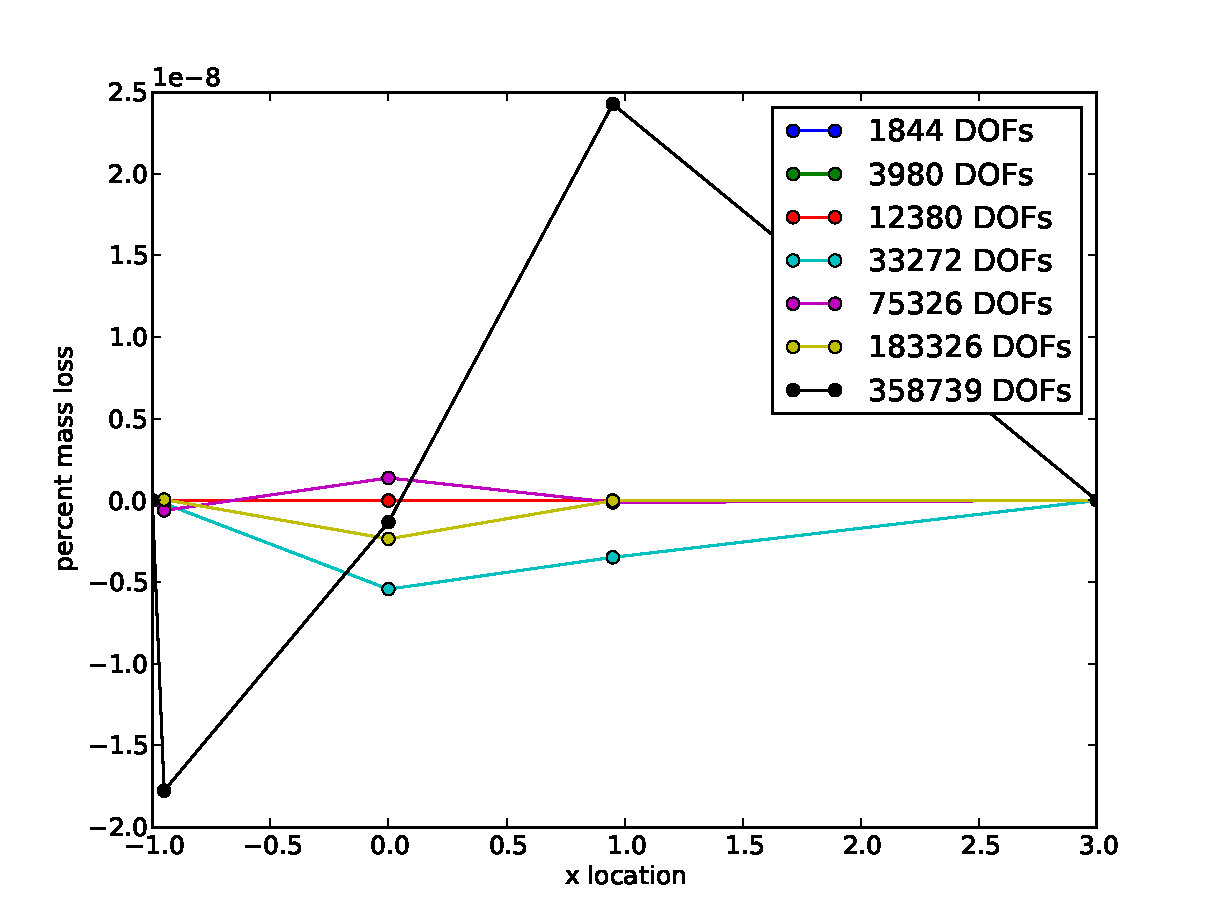
\includegraphics[width=1.1\textwidth]{StokesCylinder/MassLoss9_C.pdf}

Conservative
\end{figure}
}
\end{column}
\end{columns}
\end{frame}
\begin{comment}
\end{comment}


%===============================================================================
% NEW SLIDE
%===============================================================================
\begin{frame}
\frametitle{Numerical Experiments}
\framesubtitle{Stokes Flow Backward Facing Step}
\begin{columns}
\begin{column}{0.49\textwidth}
\only<1>{
\begin{figure}
\centering
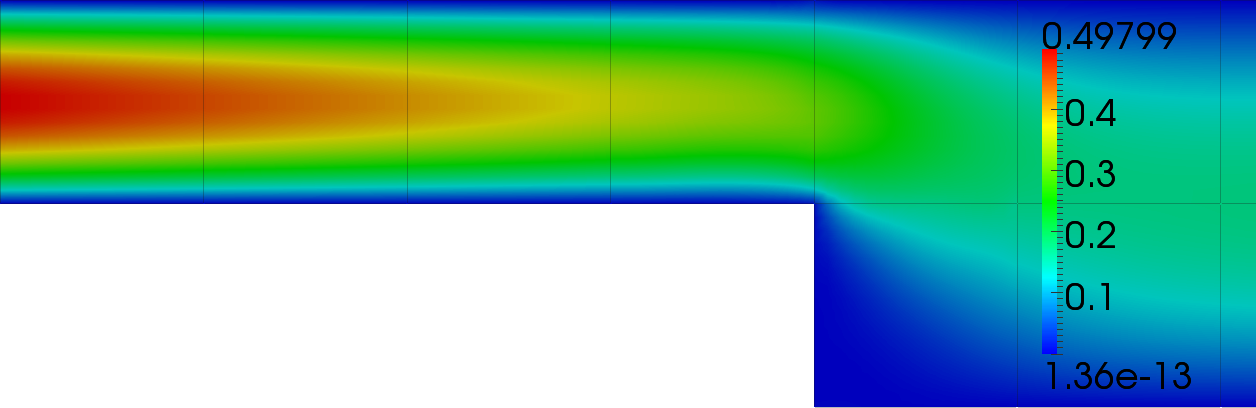
\includegraphics[width=1.0\textwidth]{StokesStep/Quartic_NC0.png}\\
\vspace{-1ex}
{\scriptsize Initial Mesh}\\
\vspace{1ex}
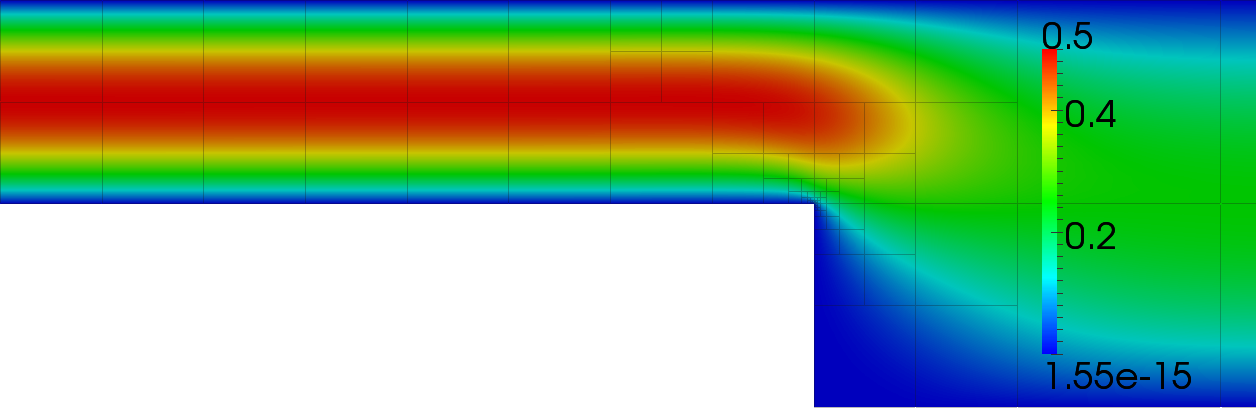
\includegraphics[width=1.0\textwidth]{StokesStep/Quartic_NC8.png}
\vspace{-1ex}
{\scriptsize 8 Refinements}
\vspace{1ex}

Nonconservative
\end{figure}
\end{column}
\begin{column}{0.49\textwidth}
\begin{figure}
\centering
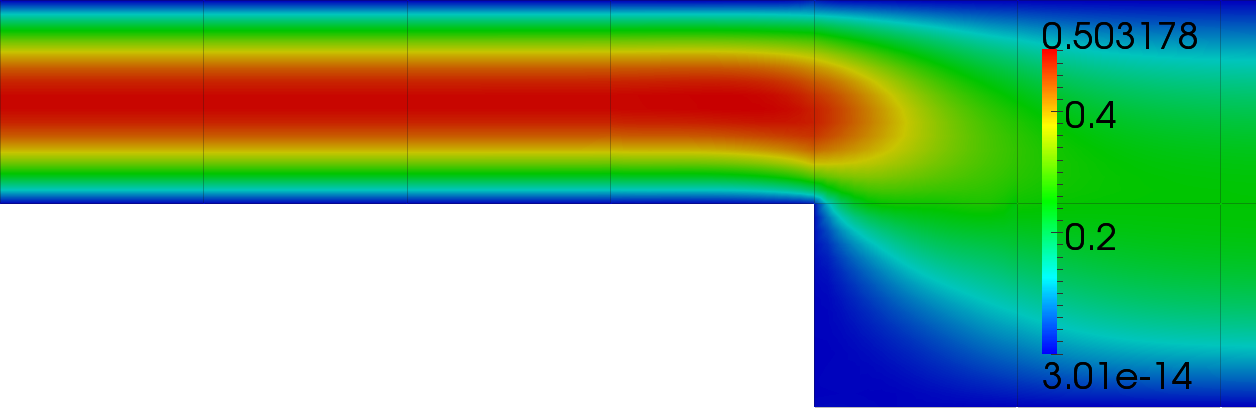
\includegraphics[width=1.0\textwidth]{StokesStep/Quartic_C0.png}\\
\vspace{-1ex}
{\scriptsize Initial Mesh}\\
\vspace{1ex}
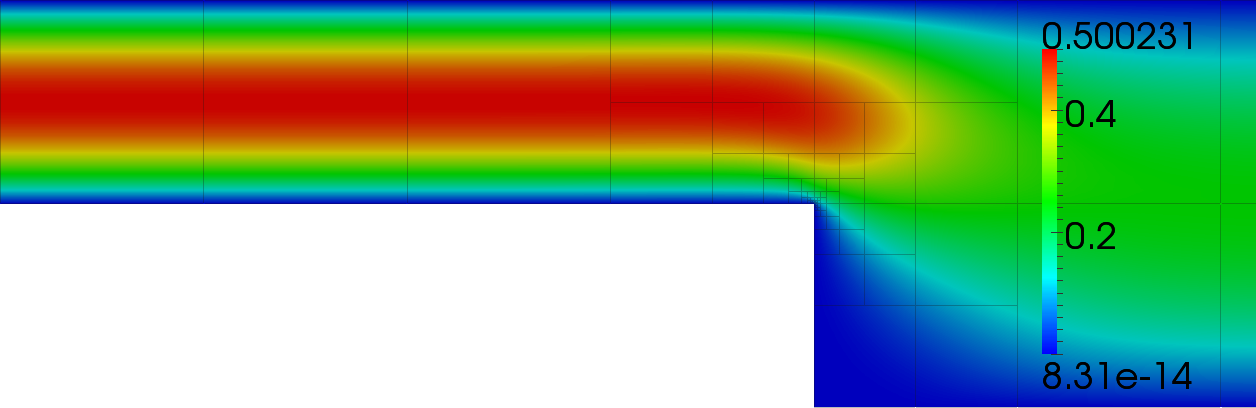
\includegraphics[width=1.0\textwidth]{StokesStep/Quartic_C8.png}
\vspace{-1ex}
{\scriptsize 8 Refinements}
\vspace{1ex}

Conservative
\end{figure}
}
\only<2>{
\begin{figure}[t]
\centering
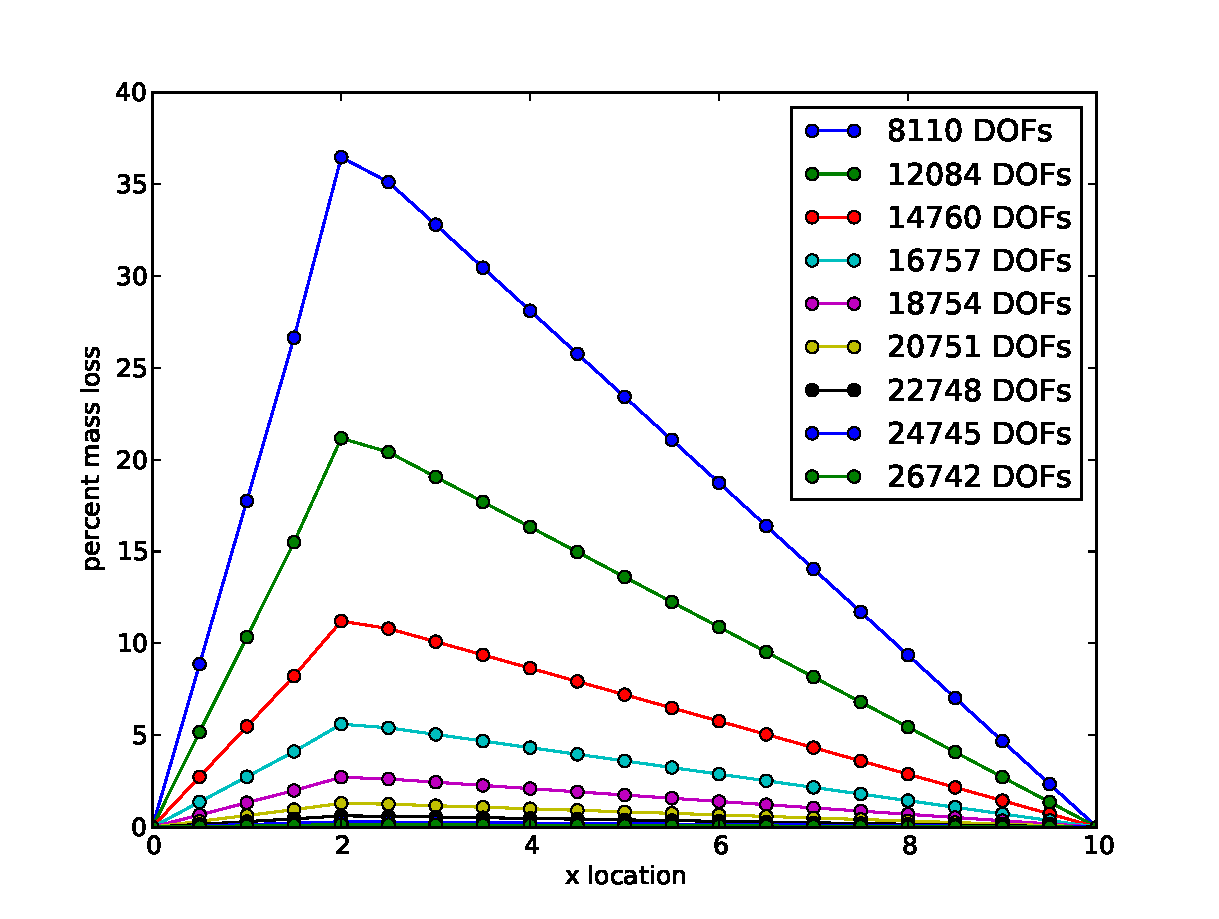
\includegraphics[width=1.1\textwidth]{StokesStep/MassLoss_NC.pdf}

Nonconservative
\end{figure}
\end{column}
\begin{column}{0.49\textwidth}
\begin{figure}[t]
\centering
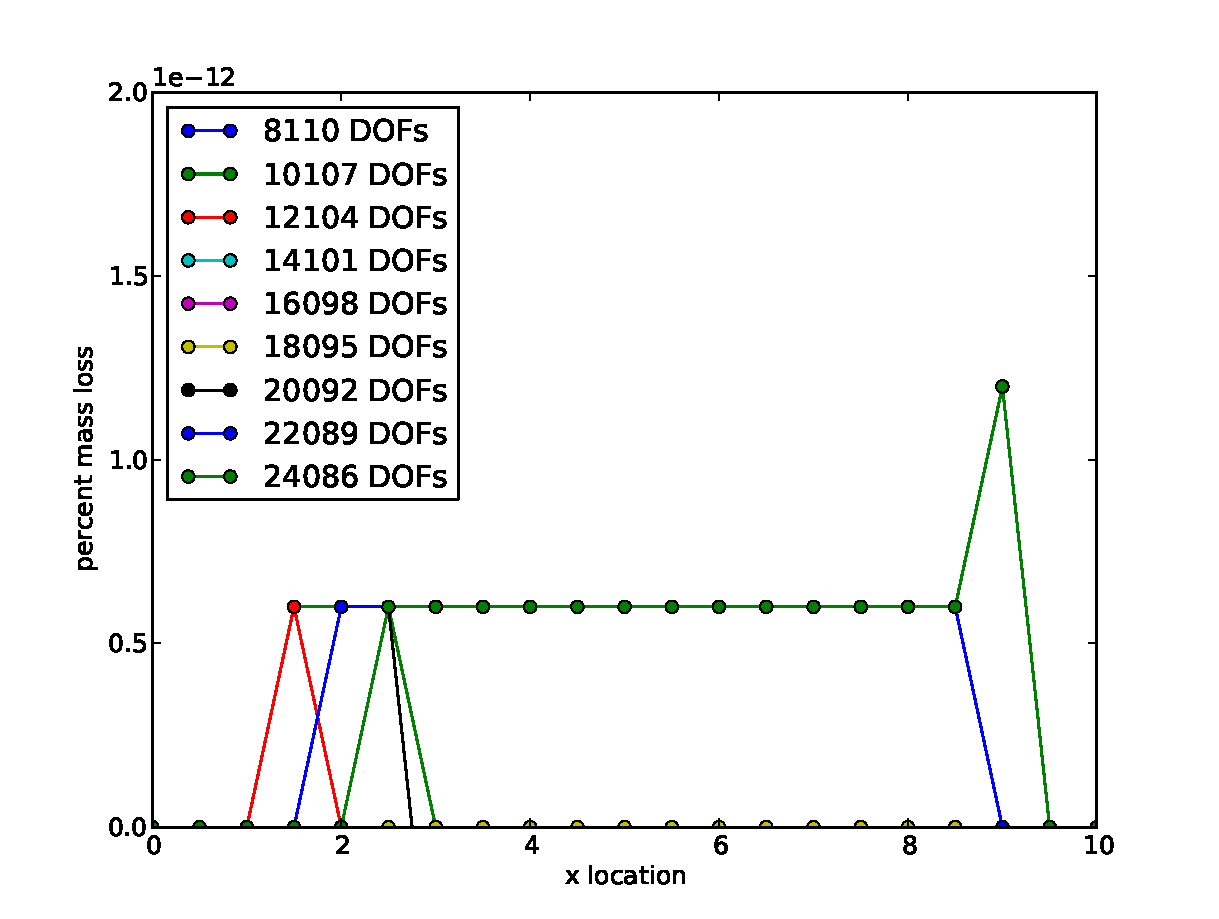
\includegraphics[width=1.1\textwidth]{StokesStep/MassLoss_C.pdf}

Conservative
\end{figure}
}
\end{column}
\end{columns}
\end{frame}
\begin{comment}
\end{comment}


\section{Space-Time DPG}
% \subsection{Mathematics}
% \subsection{Numerical Results}-
\begin{frame}[t]
\frametitle{Space-Time DPG}
\framesubtitle{Motivation}
Extends the capabilities of a DPG solver
\begin{itemize}
  \item Preserves stability and robustness of DPG method
  \item Unified treatment of space and time
  \item Local space-time adaptivity
  \begin{itemize}
    \item Small solution features require small time step
    \item Global time step not limited to smallest element
  \end{itemize}
  \item Natural framework for moving meshes
\end{itemize}
\bigskip

More computationally difficult
\begin{itemize}
  \item Solve requires $d+1$ dimensions
  \item Mesh structure more difficult
  \item Equations often first order in time but second order in space
  \item More expensive solves
\end{itemize}
\end{frame}

%   /$$   /$$                       /$$    
%  | $$  | $$                      | $$    
%  | $$  | $$  /$$$$$$   /$$$$$$  /$$$$$$  
%  | $$$$$$$$ /$$__  $$ |____  $$|_  $$_/  
%  | $$__  $$| $$$$$$$$  /$$$$$$$  | $$    
%  | $$  | $$| $$_____/ /$$__  $$  | $$ /$$
%  | $$  | $$|  $$$$$$$|  $$$$$$$  |  $$$$/
%  |__/  |__/ \_______/ \_______/   \___/  
%                                          
%                                          
%  
% ------------------------------------------------------------
\begin{frame}[t]
\frametitle{Heat Equation}
\framesubtitle{Simplest Nontrivial Space-Time Problem}  %% needed for proper positioning of the logo ...

Equation is elliptic in space, but hyperbolic in time (parabolic in space-time).
\begin{equation*}
  \frac{\partial u}{\partial t}-\epsilon\Delta u=f
\end{equation*}

This is really just a composite of Fourier's law and conservation of energy.
\begin{equation*}
\begin{aligned}
\bfsigma-\epsilon\Grad u&=0\\
\frac{\partial u}{\partial t}-\Div\bfsigma&=f
\end{aligned}
\end{equation*}

We can rewrite this in terms of a space-time divergence.
\begin{equation*}
\begin{aligned}
\frac{1}{\epsilon}\bfsigma-\Grad u&=0\\
\Divxt\vecttwo{-\bfsigma}{u}&=f
\end{aligned}
\end{equation*}
\end{frame}
\begin{comment}
Without further ado, we'll jump into the simplest representative spatial-temporal problem: the heat equation.
The interesting thing about this equation is that it is elliptic in space, but hyperbolic in time.
We can split this into two first order equations: conservation of energy and Fourier's law.
Notice that we can rewrite this as a constitutive equation and a space-time divergence.
\end{comment}

% ------------------------------------------------------------
\begin{frame}[t]
\frametitle{Heat Equation}
\framesubtitle{DPG Formulation}  %% needed for proper positioning of the logo ...
% \vspace{-2ex}
Multiply by test function and integrate by parts over space-time element K.
\begin{equation*}
\begin{aligned}
\LRp{\frac{1}{\epsilon}\bfsigma,\bftau}+\LRp{u,\Div\bftau}-\LRa{\hat u,\bftau\cdot\bfn_x}&=0\\
-\LRp{\vecttwo{-\bfsigma}{u},\Gradxt v}+\LRa{\hat t,v}&=f
\end{aligned}
\end{equation*}
\begin{columns}[t] % contents are top vertically aligned
\begin{column}[T]{0.4\textwidth} % each column can also be its own environment
where
\begin{align*}
\hat u&:=\trace(u)\\
\hat t&:=\trace(-\bfsigma)\cdot\bfn_x+\trace(u)\cdot n_t
\end{align*}
\vspace{-4ex}
\begin{itemize}
  \item Trace $\hat u$ defined on spatial boundaries
  \item Flux $\hat t$ defined on all boundaries
\end{itemize}
\end{column}
\begin{column}[T]{0.6\textwidth} % alternative top-align that's better for graphics
\vspace{-2ex}
\begin{block}{Support of Trace Variables}
\begin{tikzpicture}[line cap=round,line join=round,>=triangle 45,x=2.0cm,y=2.0cm, scale=0.6, every node/.style={scale=0.6}]
\clip(-0.7,-0.6) rectangle (5.27,2.09);
\draw (0,2)-- (0,0);
\draw (0,0)-- (1,0);
\draw (1,0)-- (4,0);
\draw (4,0)-- (5,0);
\draw (5,0)-- (5,2);
\draw (5,2)-- (3,2);
\draw (3,2)-- (2,2);
\draw (2,2)-- (0,2);
\draw (1,0)-- (1.5,1);
\draw (1.5,1)-- (2,2);
\draw (1.5,1)-- (3.5,1);
\draw (3,2)-- (3.5,1);
\draw (3.5,1)-- (4,0);
\draw (-0.21,0.9) node[anchor=south west] {$\hat u$};
\draw (4.82,0.9) node[anchor=south west] {$\hat u$};
\draw (3.5,0.45) node[anchor=south west] {$\hat u$};
\draw (1.0,0.45) node[anchor=south west] {$\hat u$};
\draw (1.5,1.4) node[anchor=south west] {$\hat u$};
\draw (3.0,1.4) node[anchor=south west] {$\hat u$};
\draw (0.05,0.9) node[anchor=south west] {$\hat t$};
\draw (1.40,0.45) node[anchor=south west] {$\hat t$};
\draw (3.79,0.45) node[anchor=south west] {$\hat t$};
\draw (2.47,1.0) node[anchor=south west] {$\hat t$};
\draw (3.33,1.4) node[anchor=south west] {$\hat t$};
\draw (1.89,1.4) node[anchor=south west] {$\hat t$};
\draw (5.07,0.9) node[anchor=south west] {$\hat t$};
\draw (4.44,0.0) node[anchor=south west] {$\hat t$};
\draw (2.46,0.0) node[anchor=south west] {$\hat t$};
\draw (0.45,0.0) node[anchor=south west] {$\hat t$};
\draw (2.44,1.7) node[anchor=south west] {$\hat t$};
\draw (0.76,1.7) node[anchor=south west] {$\hat t$};
\draw (4.21,1.7) node[anchor=south west] {$\hat t$};
\draw [->] (-0.5,-0.5) -- (-0.5,0);
\draw [->] (-0.5,-0.5) -- (0,-0.5);
\draw (-0.54,0.29) node[anchor=north west] {$t$};
\draw (0.07,-0.35) node[anchor=north west] {$x$};
\end{tikzpicture}
\end{block}
\end{column}
\end{columns}
\end{frame}
\begin{comment}
We then follow standard DPG procedure and multiply by test functions tau and v 
where tau is vector valued with dimension equal to the spatial dimension.
Then we integrate each equation by parts.
But the first equation is only integrated over spatial dimensions, so the resulting trace term is limited
to boundaries with a nonzero spatial normal component.
The integration by parts in space-time yields a flux that is defined on all boundaries, but with different
character across spatial and temporal boundaries.
\end{comment}

% ------------------------------------------------------------
\begin{frame}[t]
\frametitle{Heat equation}
\framesubtitle{Pulsed Source Problem}  %% needed for proper positioning of the logo ...
\vspace{-1ex}
\begin{columns}[t] % contents are top vertically aligned
\begin{column}[c]{0.3\textwidth} % each column can also be its own environment
% \vspace{3ex}
\begin{itemize}
  \item Initial condition $u=0$.
  \item Apply unit source $x\in[3/8,5/8]$,\\$t\in[1/4,1/2]$.
  \item Should see no temporal diffusion.
  \item Space-time adaptivity picks up areas of rapid change.
\end{itemize}
\end{column}
\begin{column}[c]{0.7\textwidth} % each column can also be its own environment
\begin{figure}[ht]
\centering
\begin{subfigure}[t]{0.45\textwidth}
\centering
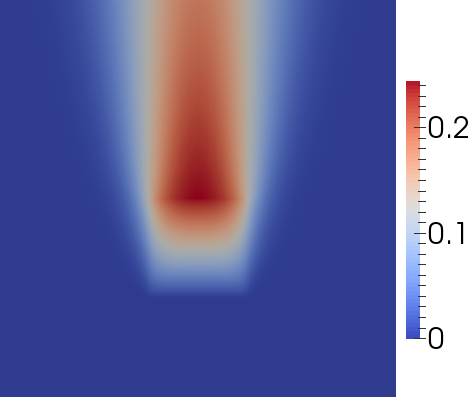
\includegraphics[height=0.8\textwidth]{SpaceTimeHeat/PulseSource/u.png}
\\$u$\\\vspace{1ex}
\end{subfigure}
\begin{subfigure}[t]{0.45\textwidth}
\centering
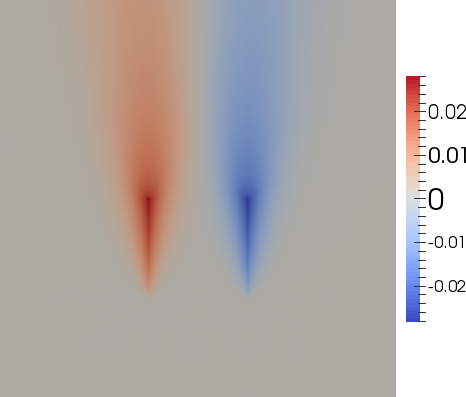
\includegraphics[height=0.8\textwidth]{SpaceTimeHeat/PulseSource/sigma.png}
\\$\sigma$\\\vspace{1ex}
\end{subfigure}
\begin{subfigure}[t]{0.45\textwidth}
\centering
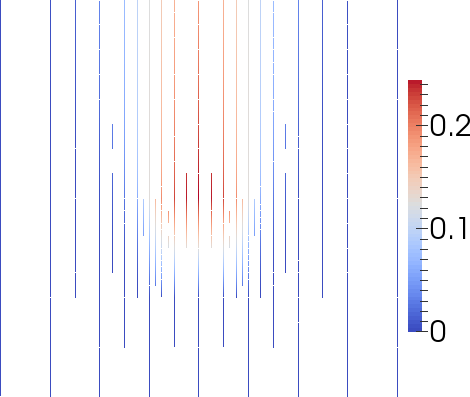
\includegraphics[height=0.8\textwidth]{SpaceTimeHeat/PulseSource/uhat.png}
\\$\hat u$
\end{subfigure}
\begin{subfigure}[t]{0.45\textwidth}
\centering
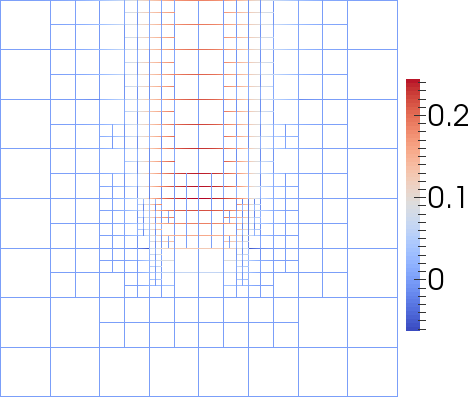
\includegraphics[height=0.8\textwidth]{SpaceTimeHeat/PulseSource/fhat.png}
\\$\hat t$
\end{subfigure}
% \caption{Pulsed space-time heat problem after 4 refinements}
\end{figure}
\end{column}
\end{columns}
\end{frame}
\begin{comment}
Here we have a very contrived example problem. 
We start with a completely zero initial condition and then turn on a unit source from t = 1/4 to t=1/2,
then watch the inputted heat diffuse over the rest of the time interval.
The key thing to watch for is making sure we don't get any heat bleeding backwards in time. 
Indeed we get  very clean start at t=1/4.
Notice also how u hat exists only on vertical boundaries, while the flux lives on the entire mesh skeleton.
We also see how the method naturally picks on on areas of rapid temporal or spatial changes and adapts to resolve them.
\end{comment}

%    /$$$$$$                                                                            /$$ /$$       /$$          
%   /$$__  $$                                                                          |__/| $$      | $$          
%  | $$  \__/  /$$$$$$  /$$$$$$/$$$$   /$$$$$$   /$$$$$$   /$$$$$$   /$$$$$$$  /$$$$$$$ /$$| $$$$$$$ | $$  /$$$$$$ 
%  | $$       /$$__  $$| $$_  $$_  $$ /$$__  $$ /$$__  $$ /$$__  $$ /$$_____/ /$$_____/| $$| $$__  $$| $$ /$$__  $$
%  | $$      | $$  \ $$| $$ \ $$ \ $$| $$  \ $$| $$  \__/| $$$$$$$$|  $$$$$$ |  $$$$$$ | $$| $$  \ $$| $$| $$$$$$$$
%  | $$    $$| $$  | $$| $$ | $$ | $$| $$  | $$| $$      | $$_____/ \____  $$ \____  $$| $$| $$  | $$| $$| $$_____/
%  |  $$$$$$/|  $$$$$$/| $$ | $$ | $$| $$$$$$$/| $$      |  $$$$$$$ /$$$$$$$/ /$$$$$$$/| $$| $$$$$$$/| $$|  $$$$$$$
%   \______/  \______/ |__/ |__/ |__/| $$____/ |__/       \_______/|_______/ |_______/ |__/|_______/ |__/ \_______/
%                                    | $$                                                                          
%                                    | $$                                                                          
%                                    |__/    

% ------------------------------------------------------------
\begin{frame}[t]
\frametitle{Compressible Navier-Stokes}
\framesubtitle{Strong Form}  %% needed for proper positioning of the logo ...
The compressible Navier-Stokes equations are
\begin{align*}
\frac{\partial}{\partial t}\svectthree{\rho}{\rho\bfu}{\rho e_0}
+\Div\svectthree{\rho\bfu}{\rho\bfu\otimes\bfu+p\bfI-\mathbb{D}}{\rho\bfu e_0+\bfu p+\bfq-\bfu\cdot\mathbb{D}}
%TODO: Possible error above. cfd-online seems to have T^T
=\svectthree{f_c}{\bff_m}{f_e}\,,
\end{align*}
where
\begin{equation*}
  \mathbb{D}=2\mu\bfS^*=2\mu\LRs{\frac{1}{2}\LRp{\Grad\bfu+\LRp{\Grad\bfu}^T}-\frac{1}{3}\Div\bfu\bfI}\,,
\end{equation*}
\begin{equation*}
  \bfq=-C_p\frac{\mu}{Pr}\Grad T\,,
\end{equation*}
and (assuming an ideal gas EOS)
\[
p=\rho R T\,.
\]
\end{frame}
\begin{comment}
Now we make a huge jump to the compressible Navier-Stokes equations, but all of the same ideas carry over.
We write our conservation equations in strong form with constitutive laws for the deviatoric stress tensor, heat flux, and pressure.
\end{comment}

% ------------------------------------------------------------
\begin{frame}[t]
\frametitle{Compressible Navier-Stokes}
\framesubtitle{First Order Space-Time Form}  %% needed for proper positioning of the logo ...
Writing this in space-time in terms of $\rho$, $\bfu$, $T$, $\mathbb{D}$, and $\bfq$:
\begin{align*}
  \mathbb{D}-\mu\LRp{\Grad\bfu+\LRp{\Grad\bfu}^T}+\frac{2\mu}{3}\Div\bfu\bfI&=0\\
  \bfq+C_p\frac{\mu}{Pr}\Grad T&=0\\
  \Divxt\vecttwo{\rho\bfu}{\rho}&=f_c\\
  \Divxt\vecttwo{\rho\bfu\otimes\bfu+\rho RT\bfI-\mathbb{D}}{\rho\bfu}&=\bff_m\\
  \Divxt\vecttwo{\rho\bfu\LRp{C_v T+\frac{1}{2}\bfu\cdot\bfu}+\bfu\rho RT+\bfq-\bfu\cdot\mathbb{D}}{\rho\LRp{C_v T+\frac{1}{2}\bfu\cdot\bfu}}&=f_e\,.
\end{align*}
\end{frame}
\begin{comment}
We follow the same course as we did for the heat equation and write this as a first order system of equations
with the conservation laws in space-time divergence form.
\end{comment}


% ------------------------------------------------------------
\begin{frame}[t]
\frametitle{Compressible Navier-Stokes}
\framesubtitle{DPG Formulation}  %% needed for proper positioning of the logo ...
Multiplying by test functions and integrating by parts:
% \scalebox{0.9}{
{
\small
\begin{align*}
  \LRp{\mathbb{D},\mathbb{S}}+\LRp{2\mu\bfu,\Div\mathbb{S}}-\LRp{\frac{2\mu}{3}\bfu,\Grad\trace{\mathbb{S}}}
  -\LRa{2\mu\hat\bfu,\mathbb{S}\bfn_x}+\LRa{\frac{2\mu}{3}\hat\bfu,\mathbb{S}\bfn_x}&=0\\
  \LRp{\bfq,\bftau}-\LRp{C_p\frac{\mu}{Pr}T,\Div\bftau}+\LRa{C_p\frac{\mu}{Pr}\hat T,\tau_n}&=0\\
  -\LRp{\vecttwo{\rho\bfu}{\rho},\Gradxt v_c}+\LRa{\hat t_c,v_c}&=\LRp{f_c,v_c}\\
  -\LRp{\vecttwo{\rho\bfu\otimes\bfu+\rho RT\bfI-\mathbb{D}}{\rho\bfu},\Gradxt\bfv_m}+\LRa{\hat\bft_m,\bfv_m}&=\LRp{\bff_m,\bfv_m}\\
  -\LRp{\vecttwo{\rho\bfu\LRp{C_v T+\frac{1}{2}\bfu\cdot\bfu}+\bfu\rho RT+\bfq-\bfu\cdot\mathbb{D}}{\rho\LRp{C_v T+\frac{1}{2}\bfu\cdot\bfu}},\Gradxt v_e}
  +\LRa{\hat t_e,v_e}&=\LRp{f_e,v_e}\,,
\end{align*}
}
% }
where $\hat u$ and $\hat T$ are spatial traces and $\hat t_c$, $\hat\bft_m$, and $\hat t_e$ are fluxes.
\end{frame}
\begin{comment}
Again we multiply by test functions and integrate by parts. In this case S is a symmetric tensor valued test function,
tau is a vector valued test function of spatial dimension, v_c and v_e are scalar valued, and v_m is vector valued matching the spatial dimension.
We've also introduced spatial traces u hat and T had and fluxes for each conservation law.
\end{comment}


% ------------------------------------------------------------
\begin{frame}[t]
\frametitle{Compressible Navier-Stokes}
\framesubtitle{Flux and Trace Variables}  %% needed for proper positioning of the logo ...
Spatial traces and fluxes are defined as follows:
\begin{equation*}
\begin{aligned}
\hat\bfu&=\trace(\bfu)\\
\hat T&=\trace(T)\\
\hat t_c&=\trace\LRp{\rho\bfu}\cdot\bfn_x
+\trace\LRp{\rho}n_t\\
\hat\bft_m&=\trace\LRp{\rho\bfu\otimes\bfu+\rho RT\bfI-\mathbb{D}}\cdot\bfn_x
+\trace\LRp{\rho\bfu} n_t\\
\hat t_e&=\trace\LRp{\rho\bfu\LRp{C_v T+\frac{1}{2}\bfu\cdot\bfu}+\bfu\rho RT+\bfq-\bfu\cdot\mathbb{D}}\cdot\bfn_x\\
&\quad+\trace\LRp{\rho\LRp{C_v T+\frac{1}{2}\bfu\cdot\bfu}}n_t\,.
\end{aligned}
\end{equation*}
\begin{block}{Linearization}
Fluxes, traces, and $\bfq$ are linear in the above bilinear form, but we need to linearize in $\rho$, $\bfu$, $T$, and $\mathbb{D}$ 
(Jacobian and residual not shown here).
\end{block}
\end{frame}
\begin{comment}
The above integration by parts gives the following definitions for the spatial traces and fluxes.
Notice the analog to the heat equation where the fluxes change nature depending on whether they are on temporal or spatial boundaries.

In the above bilinear form, the fluxes, traces, and heat flux are linear.
All of the other variables are involved in nonlinearities and will need to be linearized and solved via a Gauss-Newton iteration.
\end{comment}


%TODO: Fix test norm
% ------------------------------------------------------------
\begin{frame}[t]
\frametitle{Compressible Navier-Stokes}
\framesubtitle{Test Norm}  %% needed for proper positioning of the logo ...
\vspace{-3ex}
{
\small
\begin{align*}
&\norm{\Grad\bfv_m+\Grad v_e\otimes\tilde\bfu}^2+\norm{\Grad v_e}^2\\
+&\left\|
-\tilde\bfu\cdot\Grad v_c-\frac{\partial v_c}{\partial t}-\tilde\bfu\otimes\tilde\bfu:\Grad\bfv_m
-R\tilde T\Div\bfv_m-\tilde\bfu\cdot\frac{\partial\bfv_m}{\partial t}\right.\\
&\left.-C_v\tilde T\tilde\bfu\cdot\Grad v_e-\frac{1}{2}\tilde\bfu\cdot\tilde\bfu\tilde\bfu\cdot\Grad v_e
-R\tilde T\tilde\bfu\Grad v_e
-C_v\tilde T\frac{\partial v_e}{\partial t}-\frac{1}{2}\tilde\bfu\cdot\tilde\bfu\frac{\partial v_e}{\partial t}
\right\|^2\\
+&\left\|
-\tilde\rho\Grad v_c
-\tilde\rho\tilde\bfu\cdot\Grad\bfv_m-\tilde\rho\Grad\bfv_m\cdot\tilde\bfu
-\tilde\rho\frac{\partial\bfv_m}{\partial t}
-C_v\tilde\rho\tilde T\Grad v_e
-\frac{1}{2}\tilde\rho\tilde\bfu\cdot\tilde\bfu\Grad v_e
\right.\\
&\left.
-\frac{1}{2}\tilde\rho\tilde\bfu\cdot\Grad v_e\tilde\bfu
-\frac{1}{2}\tilde\rho\Grad v_e\cdot\tilde\bfu\tilde\bfu
-R\tilde\rho\tilde T\Grad v_e
+\tilde{\mathbb{D}}\cdot\Grad v_e
-\frac{1}{2}\tilde\rho\tilde\bfu\frac{\partial v_e}{\partial t}
-\frac{1}{2}\tilde\rho\tilde\bfu\frac{\partial v_e}{\partial t}
\right\|^2\\
+&\left\|
-R\tilde\rho\Div\bfv_m
-C_v\tilde\rho\tilde\bfu\Grad v_e
-R\tilde\rho\tilde\bfu\Grad v_e
-C_v\tilde\rho\frac{\partial v_e}{\partial t}
\right\|^2\\
+&\|\frac{1}{\mu}\mathbb{S}\|^2
+\norm{2\Div\mathbb{S}-\frac{2}{3}\Grad\trace{\mathbb{S}}}^2
+\|\frac{Pr}{C_p\mu}\bftau\|^2
+\norm{\Div\bftau}^2\\
+&\norm{v_c}^2+\norm{\bfv_m}^2+\norm{v_e}^2
\,.
\end{align*}
}
\end{frame}
\begin{comment}
Choice of test norm can be one of the most influential factors in the success of a particular DPG method.
For steady Navier-Stokes we developed a robust test norm by analogy to steady convection-diffusion.
We need to perform a similar analysis for space-time convection-diffusion, but we've found that the following norm
for Navier-Stokes seems to work better than the standard graph norm.
Essentially, we've taken the standard graph norm based off the adjoint equation and decoupled the Eulerian and viscous terms.
\end{comment}


%    /$$$$$$                  /$$                     
%   /$$__  $$                | $$                     
%  | $$  \__/  /$$$$$$   /$$$$$$$  /$$$$$$  /$$    /$$
%  |  $$$$$$  /$$__  $$ /$$__  $$ /$$__  $$|  $$  /$$/
%   \____  $$| $$$$$$$$| $$  | $$| $$  \ $$ \  $$/$$/ 
%   /$$  \ $$| $$_____/| $$  | $$| $$  | $$  \  $$$/  
%  |  $$$$$$/|  $$$$$$$|  $$$$$$$|  $$$$$$/   \  $/   
%   \______/  \_______/ \_______/ \______/     \_/    
%                                                     
%                                                     
% 
% ------------------------------------------------------------
% \begin{frame}[t]
% \frametitle{Compressible Navier-Stokes}
% \framesubtitle{Sod Shock Tube with $\mu=10^{-5}$}  %% needed for proper positioning of the logo ...
% \foreach \n in {1,...,15}
% {
% \only<\n>
% {
% \vspace{-2ex}
% \begin{figure}[ht]
% \centering

% \begin{subfigure}[c]{0.45\textwidth}
% \centering
% \includegraphics[height=0.7\textwidth]{SpaceTimeCNS/Sod1e-5/den\n.pdf}
% \end{subfigure}
% \begin{subfigure}[c]{0.45\textwidth}
% \centering
% \includegraphics[height=0.7\textwidth]{SpaceTimeCNS/Sod1e-5/vel\n.pdf}
% \end{subfigure}
% \begin{subfigure}[c]{0.45\textwidth}
% \centering
% \includegraphics[height=0.7\textwidth]{SpaceTimeCNS/Sod1e-5/pres\n.pdf}
% \end{subfigure}
% \begin{subfigure}[c]{0.45\textwidth}
% \centering
% \includegraphics[width=1\textwidth]{SpaceTimeCNS/Sod1e-5/mesh\n.png}
% \end{subfigure}
% \end{figure}
% }
% }
% \end{frame}
% \begin{comment}
% We illustrate our space-time formulation with the Sod shock tube problem starting on an initially very coarse mesh of 4
% space-time elements. 
% Traditionally the Sod shock tube is defined for the Euler equations, 
% but every numerical method that I know uses some sort of artificial viscosity to handle the shock.
% We instead just solve the problem with a small physical viscosity of order 10^-5.
% You can see that even on this extremely coarse mesh, we have a somewhat sound solution.
% Moreover, the adaptive error control of DPG begins to work to refine the mesh in the correct areas in order to
% resolve the flow features.
% We'll step through each adaptive refinement step to see how the DPG solution converges to the exact solution.
% You can see that after 14 refinement steps we are nearly right on top of the exact solution. 
% With one or two more steps we could probably completely eliminate the tiny overshoots at the shock.
% \end{comment}


% %   /$$   /$$           /$$      
% %  | $$$ | $$          | $$      
% %  | $$$$| $$  /$$$$$$ | $$$$$$$ 
% %  | $$ $$ $$ /$$__  $$| $$__  $$
% %  | $$  $$$$| $$  \ $$| $$  \ $$
% %  | $$\  $$$| $$  | $$| $$  | $$
% %  | $$ \  $$|  $$$$$$/| $$  | $$
% %  |__/  \__/ \______/ |__/  |__/
% %                                
% %                                
% % 
% % ------------------------------------------------------------
% \begin{frame}[t]
% \frametitle{Compressible Navier-Stokes}
% \framesubtitle{Noh Implosion with $\mu=10^{-3}$}  %% needed for proper positioning of the logo ...
% Infinitely strong shock propagation.
% \foreach \n in {1,...,9}
% {
% \only<\n>
% {
% \vspace{4ex}
% % \begin{figure}[ht]
% % \centering

% \begin{columns}[t] % contents are top vertically aligned
% \begin{column}[T]{0.45\textwidth} % each column can also be its own environment
% % \begin{subfigure}[c]{0.45\textwidth}
% \centering
% \includegraphics[height=1.0\textwidth]{SpaceTimeCNS/Noh1e-3/den\n.pdf}
% \end{column}
% % \end{subfigure}
% \hspace{8ex}
% \begin{column}[T]{0.45\textwidth} % each column can also be its own environment
% % \begin{subfigure}[c]{0.4\textwidth}
% \centering
% \vspace{2ex}
% \includegraphics[width=0.9\textwidth]{SpaceTimeCNS/Noh1e-3/mesh\n.png}
% \end{column}
% \end{columns}
% % \end{subfigure}
% % \end{figure}
% }
% }
% \end{frame}
% \begin{comment}
% \end{comment}


\section{Proposed Work}
\begin{frame}[t]
\frametitle{Proposed Work}
\framesubtitle{~~}  %% needed for proper positioning of the logo ...
Area A: Applicable Mathematics
\begin{itemize}
  \item Robustness analysis for space-time convection-diffusion
  \item Explore positivity preserving techniques for compressible Navier-Stokes
\end{itemize}
\bigskip

Area B: Scientific Computation
\begin{itemize}
  \item Support development of Camellia\cite{CamelliaDPG}
  \begin{itemize}
    \item Development and verification of 2D space-time simulations.
    \item Implement time slabs to decrease solve size
    \item Contribute to auxiliary features
  \end{itemize}
  \item Run parallel simulations on HPC systems at TACC and ANL
  % \item Investigate iterative solvers for DPG
\end{itemize}
\bigskip

Area C: Modeling and Applications
\begin{itemize}
  \item Revisit Carter plate solve for higher Reynolds numbers
  \item Incompressible Taylor-Green vortex problem
  \item Incompressible vortex shedding problems
  \item Possibly investigate compressible Sedov and Noh problems
\end{itemize}
\end{frame}


% ------------------------------------------------------------
% \begin{frame}[t]
% \frametitle{Conclusions and Future Work}
% \framesubtitle{~~}  %% needed for proper positioning of the logo ...
% Conclusions
% \begin{itemize}
%   \item A problem in conservation form can be transformed to a space-time divergence.
%   \item Fluxes change character from spatial to temporal boundaries.
%   \item Traces are only defined on spatial boundaries.
% \end{itemize}
% \bigskip

% Future Work
% \begin{itemize}
%   \item Proof of robustness for convection-diffusion.
%   \item Analysis of robust test norms.
%   \item Time slabs will reduce the simulation cost.
%   \item Two and three dimensions for more realistic problems.
%   \item Incompressible Navier-Stokes.
%   \item Iterative solvers for parallel scalability.
% \end{itemize}
% \end{frame}
% \begin{comment}
% It is extremely helpful to be able to write the governing equations in terms of a space-time divergence
% since that frames things in a way that we are familiar with from steady DPG.
% The oddity is that this leaves traces on temporal edges undefined, so our code needs to know not to put degrees
% of freedom there. 

% These are all very preliminary results, but they give an indication of what we can expect in the future.
% We still need to analyze the space-time convection-diffusion equation and develop robust norms in this context
% before we can extend the ideas to Navier-Stokes.
% We also have some rough work done on time-slabs which should improve the computational efficiency.
% Obviously, we are going to need to move to two and three dimensional problems in order to simulate anything of interest.
% My primary target is actually incompressible Navier-Stokes, which should be easier since we don't have to deal with shocks.
% But in 1D incompressible gives absolutely trivial solutions, so we didn't pursue it here.
% I don't know if we will get to this during my dissertation, but if we really want a scalable method, we need to address the 
% lack of preconditioners for DPG and develop a decent iterative solver.
% \end{comment}

\begin{frame}[t]
\frametitle{Bibliography}
\framesubtitle{~~}  %% needed for proper positioning of the logo ...
\bibliographystyle{plain}
{\scriptsize
\bibliography{../Papers}
}
\end{frame}

%   /$$$$$$$                      /$$                          
%  | $$__  $$                    | $$                          
%  | $$  \ $$  /$$$$$$   /$$$$$$$| $$   /$$ /$$   /$$  /$$$$$$ 
%  | $$$$$$$  |____  $$ /$$_____/| $$  /$$/| $$  | $$ /$$__  $$
%  | $$__  $$  /$$$$$$$| $$      | $$$$$$/ | $$  | $$| $$  \ $$
%  | $$  \ $$ /$$__  $$| $$      | $$_  $$ | $$  | $$| $$  | $$
%  | $$$$$$$/|  $$$$$$$|  $$$$$$$| $$ \  $$|  $$$$$$/| $$$$$$$/
%  |_______/  \_______/ \_______/|__/  \__/ \______/ | $$____/ 
%                                                    | $$      
%                                                    | $$      
%                                                    |__/ 
% \section{Backup Slides}
% \subsection{Inf-Sup}

\end{document}
